\documentclass[aspectratio=169]{beamer}

\usetheme{default}
\usefonttheme{professionalfonts}
\setbeamertemplate{navigation symbols}{}
\setbeamertemplate{itemize items}[circle]
\setbeamercolor{itemize item}{fg=white}

\setbeamerfont{title}{series=\bfseries, size=\normalfont\Large}
\setbeamercolor{title}{fg=white}

\setbeamerfont{author}{size=\normalfont\small}
\setbeamercolor{author}{fg=white}

\setbeamerfont{frametitle}{series=\bfseries, size=\normalfont}
\setbeamercolor{frametitle}{fg=white}

\setbeamerfont{framesubtitle}{size=\normalfont\large}
\setbeamercolor{framesubtitle}{fg=white}

\setbeamercolor{background canvas}{bg=black}
\setbeamercolor{normal text}{fg=white}

\setbeamercolor{local structure}{fg=white}

\usepackage[utf8]{inputenc}
\usepackage[english]{babel}
\usepackage{amsmath, amssymb}
\usepackage{amsfonts}
\usepackage{amssymb}
\usepackage{graphicx}
\usepackage[]{bm}
\usepackage[]{multimedia}
\usepackage[]{multicol}
\usepackage[squaren,Gray]{SIunits}

\graphicspath{{imgs/}}

\DeclareMathOperator*{\minimize}{minimize}
\DeclareMathOperator*{\maximize}{maximize}
\DeclareMathOperator*{\subjectto}{subject~to}


\usepackage{tikz} % Required for drawing custom shapes
\usetikzlibrary{arrows}
\usetikzlibrary{shapes.geometric, math, positioning, calc, patterns, angles, quotes}
\usetikzlibrary{patterns.meta,decorations.pathmorphing}




%\usepackage[]{listings}
\usepackage[many]{tcolorbox}
\tcbuselibrary{listings}

%% \definecolor{codegreen}{rgb}{0,0.8,0}
%% \definecolor{codegray}{rgb}{0.5,0.5,0.5}
%% %\definecolor{codepurple}{rgb}{0.58,0,0.82}
%% \definecolor{codepurple}{rgb}{0,0.8,0}
%% \definecolor{backcolour}{rgb}{0.0, 0.0, 0.0}

\definecolor{codegreen}{rgb}{0,0.6,0}
\definecolor{codered}{rgb}{0.6,0.1,0}
\definecolor{codegray}{rgb}{0.5,0.5,0.5}
\definecolor{codepurple}{rgb}{0.58,0,0.82}
\definecolor{backcolour}{rgb}{0, 0, 0}
\definecolor{lightgray}{gray}{0.95}
\definecolor{codeblue}{rgb}{0.117,0.403,0.713}

\newcounter{ipythcntr}
\renewcommand{\theipythcntr}{\texttt{[\arabic{ipythcntr}]}}
\newcommand{\ipin}[1][]{
  \stepcounter{ipythcntr}
  \hspace{-10pt}
  \color{codeblue}In  \theipythcntr}
\newcommand{\ipout}[1][\theipythcntr]{
  \hspace{-10pt}
  \color{codered}Out \theipythcntr}

\lstdefinestyle{mystyle}{
  language=Python,
  moredelim=[is][\ipin]{In[}{]},
  moredelim=[is][\ipout]{Out[}{]},
  backgroundcolor=\color{backcolour},
  commentstyle=\color{codegreen},
  keywordstyle=\color{magenta},
  numberstyle=\tiny\color{codegray},
  stringstyle=\color{codepurple},
  basicstyle=\ttfamily\footnotesize,
  breakatwhitespace=false,
  breaklines=true,
  captionpos=b,
  keepspaces=true,
  numbers=left,
  numbersep=5pt,
  showspaces=false,
  showstringspaces=false,
  showtabs=false,
  tabsize=2,
}

\lstset{style=mystyle}


\title{Accelerating Jacobi solvers}
\author{Jean-Christophe LOISEAU}
\institute{Arts \& Métiers Institute of Technology, January 2022}
\date{}

\begin{document}





\frame{\titlepage}





\begin{frame}

  \begin{overprint}
    \onslide<1>
    \huge
    \[
    \bm{Ax} = \bm{b}
    \]

    \onslide<2>
    \huge
    \[
    \bm{x} = \bm{A}^{-1} \bm{b}
    \]

    \bigskip

    \flushright
    \small
    Provided $\bm{A}$ is invertible\ldots
  \end{overprint}
  \vspace{-1cm}
\end{frame}

{
  \setbeamercolor{background canvas}{bg=white}
  \frame{
    \vfill
    \centering
    \vfill
  }
}

\begin{frame}
  \centering
  \textbf{Unsteady heat equation}
  
  \medskip
  
  \begin{overprint}
    \onslide<1>
    \large
    \[
    \dfrac{\partial \theta}{\partial t} = \kappa \nabla^2 \theta
    \]
    
    \onslide<2>
    \large
    \[
    \left( \bm{I} - \dfrac{\kappa \Delta t}{2} \nabla^2 \right) \theta_{k+1} = \left( \bm{I} + \dfrac{\kappa \Delta t}{2} \nabla^2 \right) \theta_k
    \]
    
    
    \onslide<3>
    \[
    \underbrace{
      \left( \bm{I} - \dfrac{\kappa \Delta t}{2} \nabla^2 \right)}_{\textbf{Helmholtz operator}}
    \theta_{k+1} = \left( \bm{I} + \dfrac{\kappa \Delta t}{2} \nabla^2 \right) \theta_k
    \]
  \end{overprint}
  
  \vspace{-1cm}
\end{frame}

{
  \usebackgroundtemplate{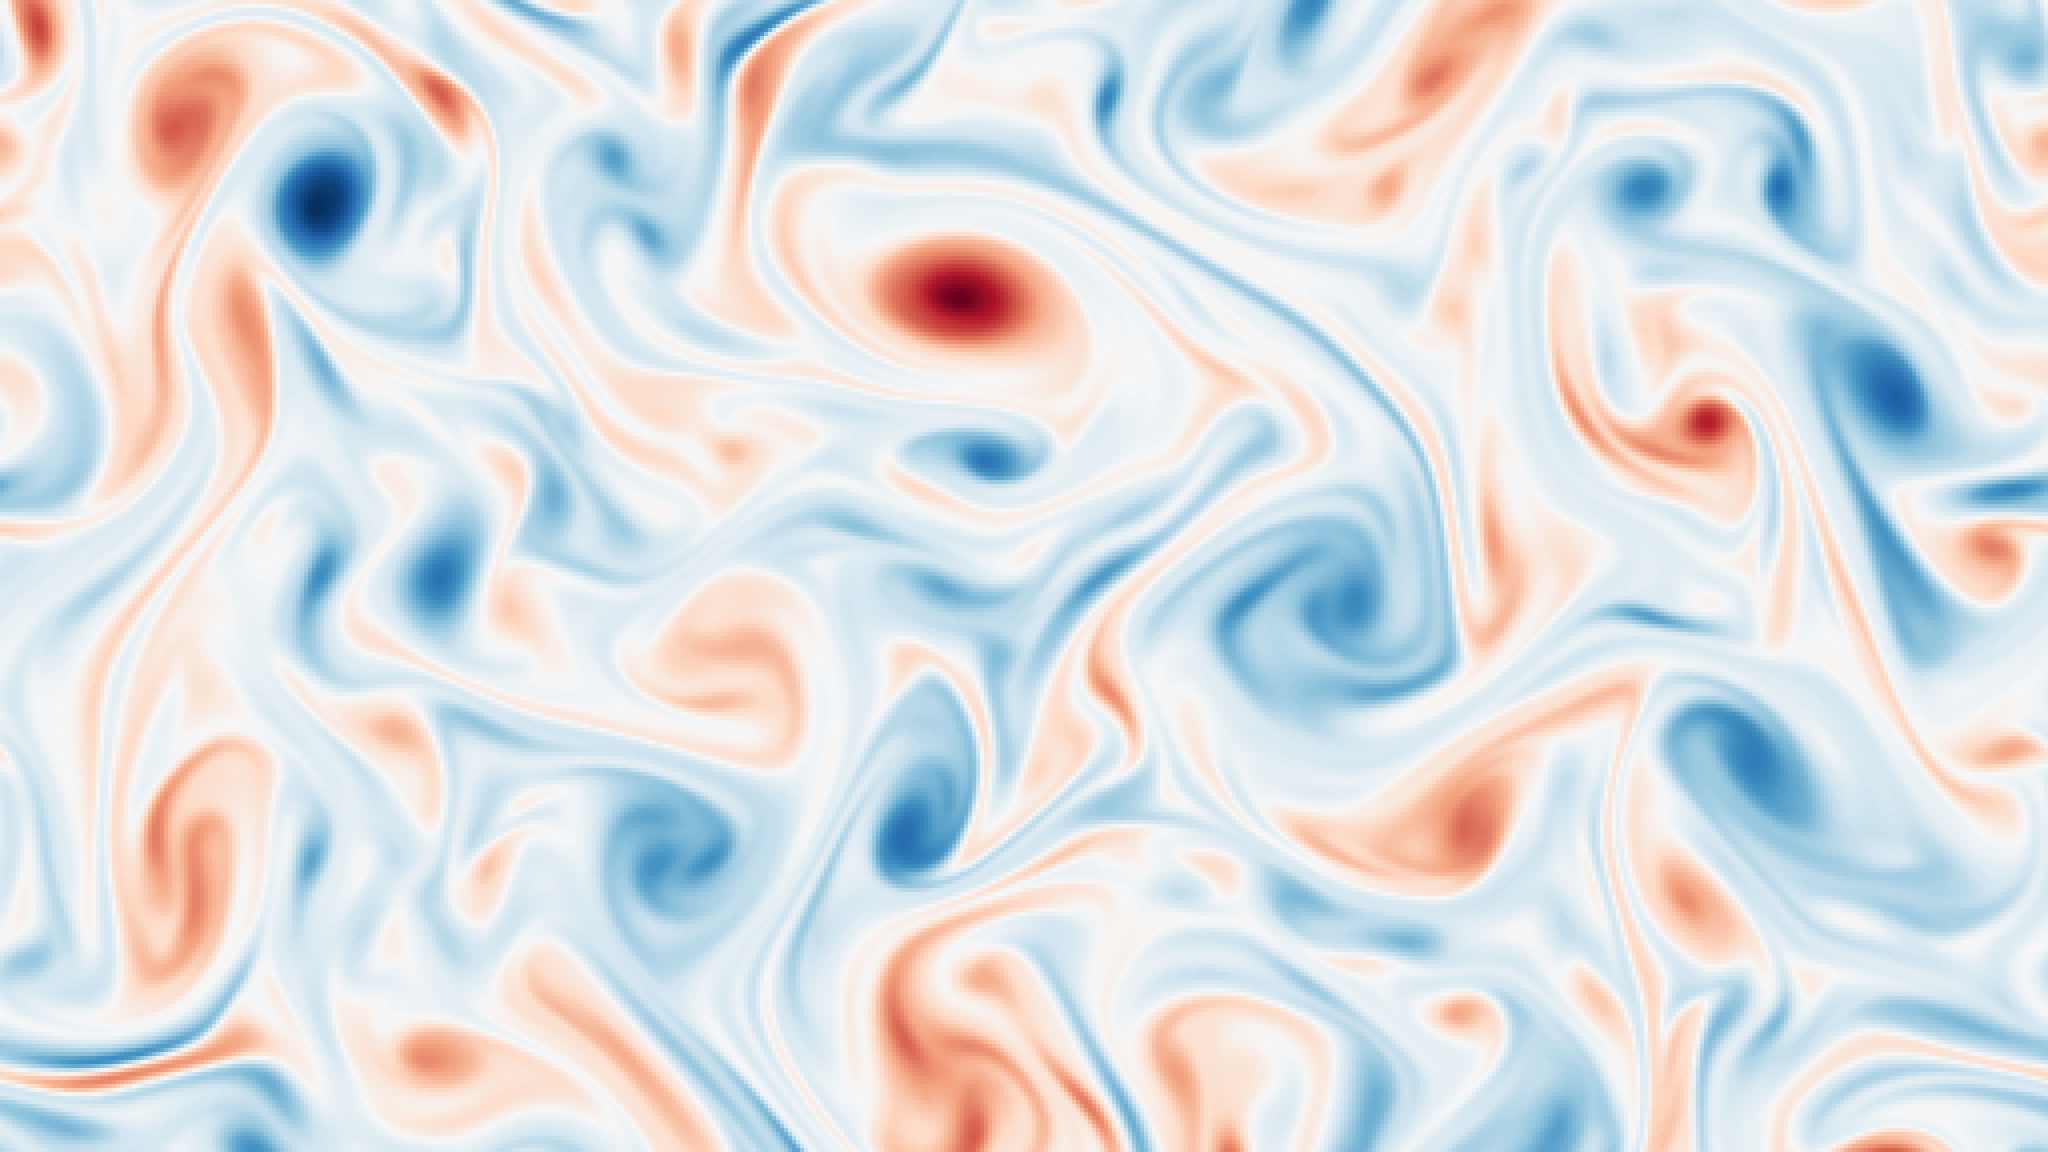
\includegraphics[width=\paperwidth]{2D_turb}}
  \begin{frame}[plain]
  \end{frame}
}

\begin{frame}
  \begin{minipage}{.68\textwidth}
    \centering
    \textbf{2D Navier-Stokes equations}

    \medskip

    \begin{overprint}
      \onslide<1>
      \large
      \[
      \dfrac{\partial \omega}{\partial t} + J(\omega, \psi) = \dfrac{1}{Re} \nabla^2 \omega
      \]

      \onslide<2>
      \large
      \[
      \nabla^2 \psi = - \omega
      \]

      \onslide<3>
      \large
      \[
      \underbrace{\nabla^2 \psi = - \omega}_{\textbf{Poisson equation}}
      \]
    \end{overprint}
  \end{minipage}%
  \hfill
  \begin{minipage}{.28\textwidth}
    \movie[width=\textwidth, autostart, loop]{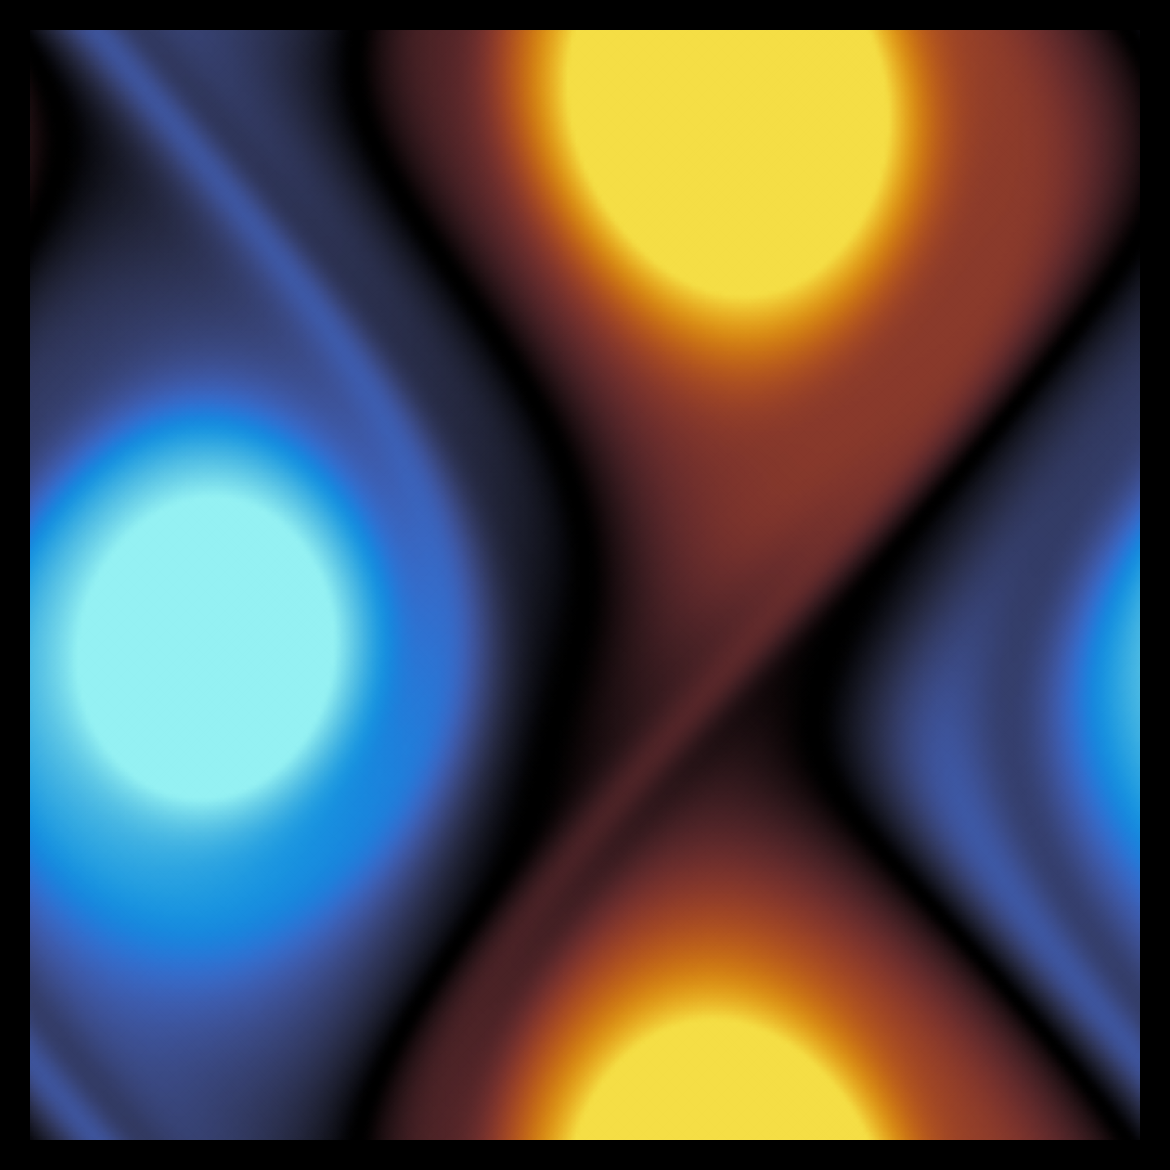
\includegraphics[width=\textwidth]{2D_turbulence}}{imgs/2D_turbulence.mp4}
  \end{minipage}
  \vspace{-1cm}
\end{frame}

\begin{frame}[t, c]{Some assumptions made throughout this talk}{}
  \begin{minipage}{.58\textwidth}
    \begin{overprint}
      \onslide<1>
      Matrices to be inverted result from the discretization of differential operators (e.g. Laplacian).

      \onslide<2>
      Choice of discretization results in \alert{\textbf{sparse}}, \alert{\textbf{banded}} and \alert{\textbf{diagonally-dominant}} matrices.

      \onslide<3>
      Your numerical solver already has a \alert{\textbf{Jacobi method}} available (or it can easily be implemented).
    \end{overprint}
  \end{minipage}%
  \hfill
  \begin{minipage}{.38\textwidth}
    \begin{overprint}
      \onslide<1>
      \[
      \dfrac{d^2 f}{dx^2} \simeq \dfrac{f_{i+1} - 2f_i + f_{i-1}}{\Delta x^2}
      \]

      \onslide<2>
      \[
      \begin{bmatrix}
        \bm{A}_{11} & \bm{A}_{12} &  &  &  \\
        \bm{A}_{21} & \bm{A}_{22} & \bm{A}_{23} &  & \\
         & \bm{A}_{32} & \bm{A}_{33} & \bm{A}_{34} &  \\
         &  & \bm{A}_{43} & \bm{A}_{44} & \bm{A}_{45} \\
          &  &  & \bm{A}_{54} & \bm{A}_{55}
      \end{bmatrix}
      \]
    \end{overprint}
  \end{minipage}

  \vspace{-1cm}
\end{frame}

\begin{frame}[t, c]{Direct linear solvers}{}
  \begin{minipage}{.68\textwidth}
    \centering
    \textbf{LU decomposition:} $\bm{A} \in GL(n)$
    \medskip
    \Large
    \[
    \bm{Ax} = \bm{b}
    \]
  \end{minipage}%
  \hfill
  \begin{minipage}{.28\textwidth}
  \end{minipage}
\end{frame}

{
  \setbeamercolor{background canvas}{bg=white}
  \frame{
    \vfill
    \centering
    \color{black}
    \large
    \[
    \underbrace{
    \begin{bmatrix}
      a_{11} & a_{12} & a_{13} & a_{14} \\
      a_{21} & a_{22} & a_{23} & a_{24} \\
      a_{31} & a_{32} & a_{33} & a_{34} \\
      a_{41} & a_{42} & a_{43} & a_{44} \\
    \end{bmatrix}}_{\bm{A}}
    =
    \underbrace{
    \begin{bmatrix}
      l_{11} &  &  &  \\
      l_{21} & l_{22} &  &  \\
      l_{31} & l_{32} & l_{33} &  \\
      l_{41} & l_{42} & l_{43} & l_{44} \\
    \end{bmatrix}}_{\bm{L}}
    \underbrace{
    \begin{bmatrix}
      u_{11} & u_{12} & u_{13} & u_{14} \\
       & u_{22} & u_{23} & u_{24} \\
       &  & u_{33} & u_{34} \\
       &  &  & u_{44} \\
    \end{bmatrix}}_{\bm{U}}
    \]
    \vfill
  }
}


\begin{frame}[t, c]{Direct linear solvers}{}
  \begin{minipage}{.68\textwidth}
    \centering
    \textbf{LU decomposition:} $\bm{A} \in GL(n)$

    \medskip

    \begin{overprint}
      \onslide<1>
      \Large
      \[
      \bm{LUx} = \bm{b}
      \]

      \onslide<2>
      \Large
      \[
      \bm{Ux} = \bm{L}^{-1} \bm{b}
      \]

      \onslide<3>
      \Large
      \[
      \bm{x} = \bm{U}^{-1} \bm{L}^{-1} \bm{b}
      \]

      \onslide<4>
      \Large
      \[
      \bm{x} = \bm{A}^{-1} \bm{b}
      \]
    \end{overprint}
  \end{minipage}%
  \hfill
  \begin{minipage}{.28\textwidth}
    \begin{overprint}
      \onslide<1>
      \[\mathcal{O}(n^3)\]
      \vspace{-1cm}

      \onslide<2-3>
      \[\mathcal{O}(n^2)\]
      \vspace{-1cm}
    \end{overprint}
  \end{minipage}
\end{frame}

\begin{frame}[t, c]{Direct linear solvers}{}
  \vfill
  \centering
  \begin{tabular}{ccc}
    ~ & \textbf{Factorization} & \textbf{Triangular solve} \\ \\
    \hline \\
    \textbf{Complexity} & {\color{red}$\mathcal{O}(n^3)$} & $\mathcal{O}(n^2)$
  \end{tabular}
  \vfill
\end{frame}


%% \begin{frame}[t, c]{Direct linear solvers}{}
%%   \begin{minipage}{.68\textwidth}
%%     \centering
%%     \textbf{Cholesky decomposition:} $\bm{A} \in S_{++}(n)$
%%     \medskip
%%     \Large
%%     \[
%%     \bm{Ax} = \bm{b}
%%     \]
%%   \end{minipage}%
%%   \hfill
%%   \begin{minipage}{.28\textwidth}
%%   \end{minipage}
%% \end{frame}

%% {
%%   \setbeamercolor{background canvas}{bg=white}
%%   \frame{
%%     \vfill
%%     \centering
%%     \color{black}
%%     \large
%%     \[
%%     \underbrace{
%%     \begin{bmatrix}
%%       a_{11} & a_{12} & a_{13} & a_{14} \\
%%       a_{12} & a_{22} & a_{23} & a_{24} \\
%%       a_{13} & a_{23} & a_{33} & a_{34} \\
%%       a_{14} & a_{24} & a_{34} & a_{44} \\
%%     \end{bmatrix}}_{\bm{A}}
%%     =
%%     \underbrace{
%%     \begin{bmatrix}
%%       l_{11} &  &  &  \\
%%       l_{21} & l_{22} &  &  \\
%%       l_{31} & l_{32} & l_{33} &  \\
%%       l_{41} & l_{42} & l_{43} & l_{44} \\
%%     \end{bmatrix}}_{\bm{L}}
%%     \underbrace{
%%     \begin{bmatrix}
%%       l_{11} & l_{21} & l_{31} & l_{41} \\
%%       & l_{22} & l_{32} & l_{42} \\
%%       &  & l_{33} & l_{43} \\
%%       &  &  & l_{44} \\
%%     \end{bmatrix}}_{\bm{L}^T}
%%     \]
%%     \vfill
%%   }
%% }

%% \begin{frame}[t, c]{Direct linear solvers}{}
%%   \begin{minipage}{.68\textwidth}
%%     \centering
%%     \textbf{Cholesky decomposition:} $\bm{A} \in S_{++}(n)$

%%     \medskip

%%     \begin{overprint}
%%       \onslide<1>
%%       \Large
%%       \[
%%       \bm{LL}^T\bm{x} = \bm{b}
%%       \]

%%       \onslide<2>
%%       \Large
%%       \[
%%       \bm{L}^T \bm{x} = \bm{L}^{-1} \bm{b}
%%       \]

%%       \onslide<3>
%%       \Large
%%       \[
%%       \bm{x} = \bm{L}^{-T} \bm{L}^{-1} \bm{b}
%%       \]

%%       \onslide<4>
%%       \Large
%%       \[
%%       \bm{x} = \bm{A}^{-1} \bm{b}
%%       \]
%%     \end{overprint}
%%   \end{minipage}%
%%   \hfill
%%   \begin{minipage}{.28\textwidth}
%%     \begin{overprint}
%%       \onslide<1>
%%       \[\mathcal{O}(n^3)\]
%%       \vspace{-1cm}

%%       \onslide<2-3>
%%       \[\mathcal{O}(n^2)\]
%%       \vspace{-1cm}
%%     \end{overprint}
%%   \end{minipage}
%% \end{frame}


%% \begin{frame}[t, c]{Direct linear solvers}{}
%%   \vfill
%%   \centering
%%   \begin{tabular}{ccc}
%%     ~ & \textbf{Factorization} & \textbf{Triangular solve} \\ \\
%%     \hline \\
%%     \textbf{Complexity} & {\color{red}$\mathcal{O}(n^3)$} & $\mathcal{O}(n^2)$
%%   \end{tabular}
%%   \vfill
%% \end{frame}

\begin{frame}[t, c]{Krylov-based solvers}{}
  \begin{minipage}{.68\textwidth}
    \centering
    \textbf{Krylov methods}
    \Large
    \[
    \minimize_{\bm{x} \in \bm{K}} \quad \| \bm{Ax} - \bm{b} \|
    \]
  \end{minipage}%
  \hfill
  \begin{minipage}{.28\textwidth}
    \begin{overprint}
      \onslide<1>
      \centering
      \vfill
      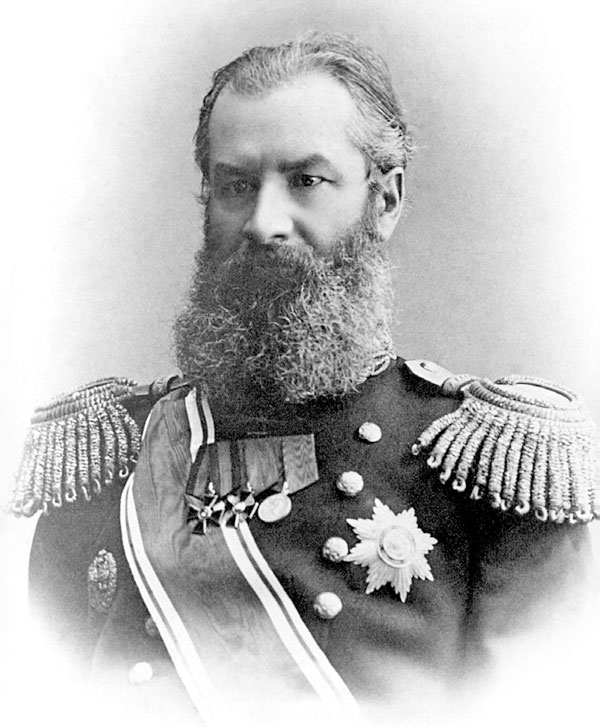
\includegraphics[width=\textwidth]{alexey_krylov}

      \small
      Alexey Krylov (1864-1945)
      \vfill

      \onslide<2>
      \vfill
      Conjugate Gradient \\
      BiCGSTAB \\
      GMRES \\
      MINRES \\
      ORTHORES \\
      QMR \\
      TFQMR \\
      Arnoldi \\
      Lancsoz \\
      \ldots
      \vfill
    \end{overprint}
  \end{minipage}
\end{frame}

\begin{frame}[t, c]{Krylov-based solvers}{}
  \vfill
  \centering
  \begin{tabular}{ccc}
    ~ & \textbf{Krylov subspace with} $\textrm{dim } \bm{K} = k$ & \textbf{Direct inversion} \\ \\
    \hline \\
    \textbf{Complexity} & {\color{red} $\mathcal{O}(kn^2)$} & $\mathcal{O}(k^3)$
  \end{tabular}
  \vfill
\end{frame}


{
  \setbeamercolor{background canvas}{bg=white}
  \frame{
    \vfill
    \centering
        {\Large
          {\color{black} \textbf{Jacobi-based methods}}
        }

        \medskip

        {\large
          {\color{gray} \textbf{Text-book material}}
        }
        \vfill
  }
}

\begin{frame}[t, c]{Jacobi method}{}
  \begin{minipage}{.68\textwidth}
    \begin{overprint}
      \onslide<1>
      Taught in every class on numerical linear algebra.
      Extremely simple to implement and easy to study theoretically.

      \onslide<2>
      Barely used in high-performance computing because of its poor convergence speed as $n$ increases.
    \end{overprint}
  \end{minipage}%
  \hfill
  \begin{minipage}{.28\textwidth}
    \centering
    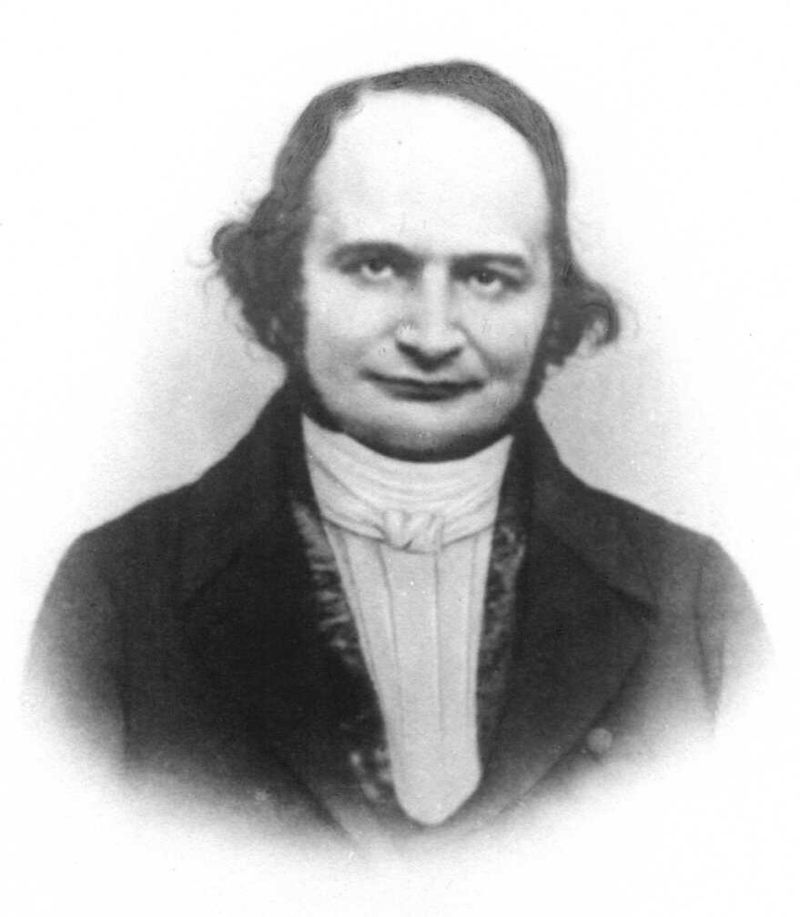
\includegraphics[width=\textwidth]{carl_jacobi}

    \small
    Carl Jacob Jacobi (1804-1851)
  \end{minipage}
\end{frame}

{
  \setbeamercolor{background canvas}{bg=white}
  \frame{
    \vfill
    \centering
    \large
    \color{black}
    \[
    \underbrace{
      \begin{bmatrix}
        a_{11} & a_{12} & a_{13} & a_{14} \\
        a_{21} & a_{22} & a_{23} & a_{24} \\
        a_{31} & a_{32} & a_{33} & a_{34} \\
        a_{41} & a_{42} & a_{43} & a_{44} \\
    \end{bmatrix}}_{\bm{A}}
    =
    \underbrace{
      \begin{bmatrix}
        a_{11} &   &   &   \\
          & a_{22} &   &   \\
          &   & a_{33} &   \\
          &   &   & a_{44} \\
    \end{bmatrix}}_{\bm{D}}
    +
    \underbrace{
      \begin{bmatrix}
          & a_{12} & a_{13} & a_{14} \\
        a_{21} &   & a_{23} & a_{24} \\
        a_{31} & a_{32} &   & a_{34} \\
        a_{41} & a_{42} & a_{43} &   \\
    \end{bmatrix}}_{\bm{R}}
    \]
  }
}

\begin{frame}
  \begin{overprint}
    \onslide<1>
    \Large
    \[
    \bm{Ax} = \bm{b}
    \]

    \onslide<2>
    \Large
    \[
    \left( \bm{D} + \bm{R} \right) \bm{x} = \bm{b}
    \]

    \onslide<3>
    \Large
    \[
    \bm{Dx} = \bm{b} - \bm{Rx}
    \]

    \onslide<4>
    \Large
    \[
    \bm{x}_{k+1} = \bm{D}^{-1} \left( \bm{b} - \bm{Rx}_k \right)
    \]

    \onslide<5>
    \Large
    \[
    \bm{x}_{k+1} = \bm{x}_k + \bm{D}^{-1} \left( \bm{b} - \bm{Ax}_k \right)
    \]

  \end{overprint}

  \vspace{-1cm}
\end{frame}

\begin{frame}
    \centering
    \textbf{Error dynamics :}    \(    \bm{e}_{k+1} = \left( \bm{I} - \bm{D}^{-1} \bm{A} \right) \bm{e}_k    \)
    
    \bigskip
    
    Jacobi method converges provided $\rho \left(\bm{I} - \bm{D}^{-1} \bm{A} \right) < 1$.

    \vspace{-1cm}
\end{frame}

{
  \setbeamercolor{background canvas}{bg=white}
  \begin{frame}[fragile]{}{}
    \vfill
    \begin{lstlisting}[backgroundcolor=\color{white}, basicstyle=\ttfamily\footnotesize\color{black}]
      import numpy as np

      def jacobi_solver(A, b, x, maxiter, tol):

          # --> Extrait la diagonale de A.
          invD = 1.0 / np.diag(A)

          # --> Iteration de Jacobi.
          for k in range(maxiter):
              r = b - A @ x
              if np.linalg.norm(r) < tol:
                  break
              x -= invD * r

          return x
    \end{lstlisting}
    \vfill
  \end{frame}
}

\begin{frame}[t, c]{Gauss-Seidel method}{}
  \begin{minipage}{.68\textwidth}
    \begin{overprint}
      \onslide<1>
      Taught in every class on numerical linear algebra.
      Extremely simple to implement and easy to study theoretically.

      \onslide<2>
      Better convergence properties than the Jacobi method albeit not enough to be really useful for HPC applications.
    \end{overprint}
  \end{minipage}%
  \hfill
  \begin{minipage}{.28\textwidth}
    \centering
    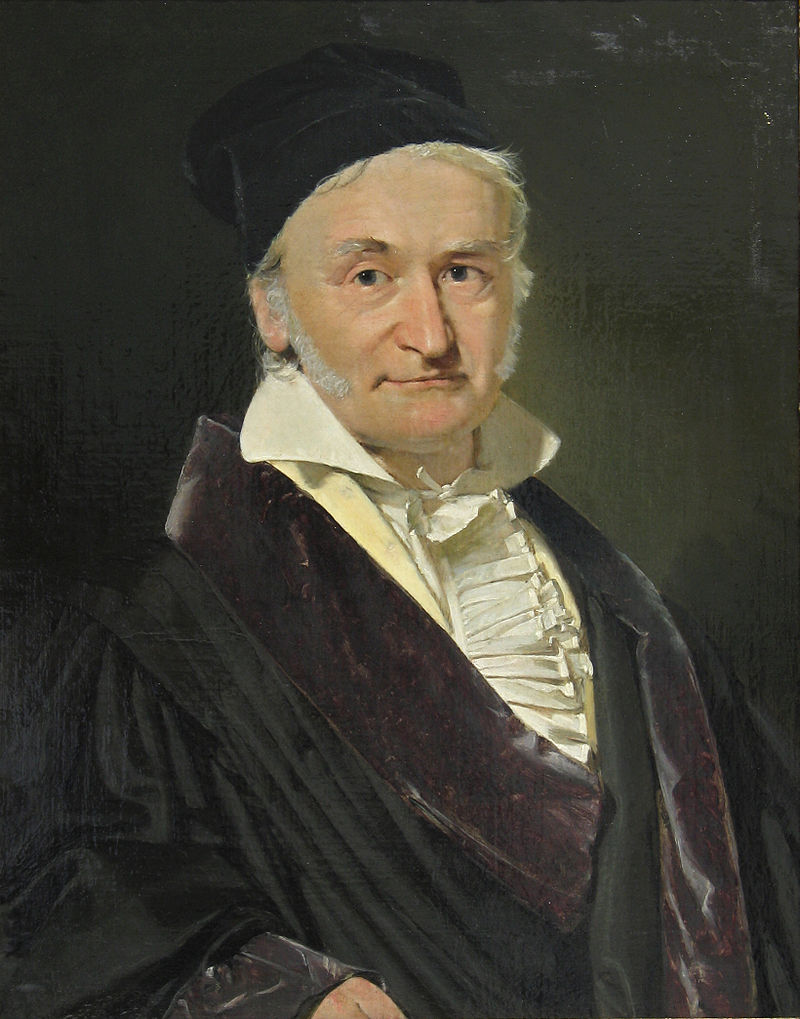
\includegraphics[height=.4\textheight]{peinture_gauss}

    \bigskip

    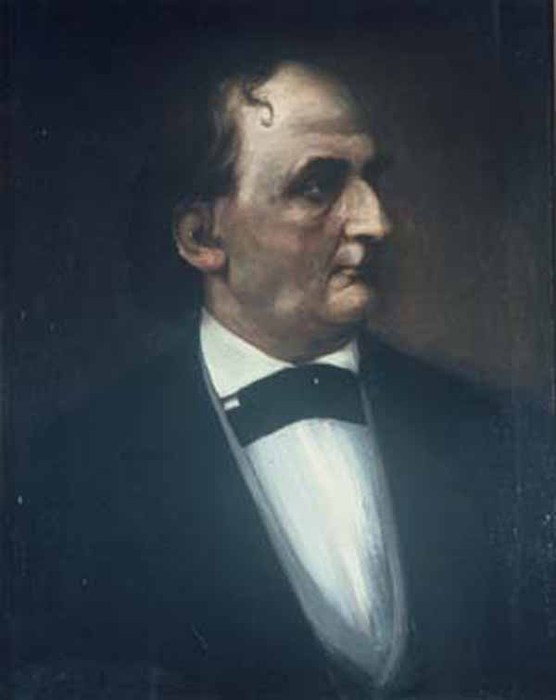
\includegraphics[height=.4\textheight]{peinture_seidel}
  \end{minipage}
\end{frame}

{
  \setbeamercolor{background canvas}{bg=white}
  \frame{
    \vfill
    \centering
    \large
    \color{black}
    \[
    \underbrace{
      \begin{bmatrix}
        a_{11} & a_{12} & a_{13} & a_{14} \\
        a_{21} & a_{22} & a_{23} & a_{24} \\
        a_{31} & a_{32} & a_{33} & a_{34} \\
        a_{41} & a_{42} & a_{43} & a_{44} \\
    \end{bmatrix}}_{\bm{A}}
    =
    \underbrace{
      \begin{bmatrix}
        a_{11} &   &   &   \\
        a_{21} & a_{22} &   &   \\
        a_{32} & a_{32} & a_{33} &   \\
        a_{41} & a_{42} & a_{43} & a_{44} \\
    \end{bmatrix}}_{\bm{L} + \bm{D}}
    +
    \underbrace{
      \begin{bmatrix}
          & a_{12} & a_{13} & a_{14} \\
          &   & a_{23} & a_{24} \\
          &   &   & a_{34} \\
          &   &   &   \\
    \end{bmatrix}}_{\bm{U}}
    \]
  }
}

\begin{frame}
  \begin{overprint}
    \onslide<1>
    \Large
    \[
    \bm{Ax} = \bm{b}
    \]

    \onslide<2>
    \Large
    \[
    \left( \bm{L} + \bm{D} + \bm{U} \right) \bm{x} = \bm{b}
    \]

    \onslide<3>
    \Large
    \[
    \left( \bm{L} + \bm{D} \right) \bm{x} = \bm{b} - \bm{Ux}
    \]

    \onslide<4>
    \Large
    \[
    \bm{x}_{k+1} = \left( \bm{L} + \bm{D} \right)^{-1} \left( \bm{b} - \bm{Ux}_k \right)
    \]

    \onslide<5>
    \Large
    \[
    \bm{x}_{k+1} = \bm{x}_k + \left( \bm{L} + \bm{D} \right)^{-1} \left( \bm{b} - \bm{Ax}_k \right)
    \]

  \end{overprint}

  \vspace{-1cm}
\end{frame}

\begin{frame}
  \centering
  \textbf{Error dynamics :} \( \bm{e}_{k+1} = \left( \bm{I} - \bm{M}^{-1} \bm{A} \right) \bm{e}_k \)
  
  \bigskip
  
  Gauss-Seidel method converges provided $\rho \left(\bm{I} - \bm{M}^{-1} \bm{A} \right) < 1$.

  \vspace{-1cm}
\end{frame}

{
  \setbeamercolor{background canvas}{bg=white}
  \begin{frame}[fragile]{}{}
    \vfill
    \begin{lstlisting}[backgroundcolor=\color{white}, basicstyle=\ttfamily\footnotesize\color{black}]
      import numpy as np
      from scipy.linalg import solve_triangular

      def gauss_seidel(A, b, x0, maxiter, tol):
          # --> Extrait L et U.
          L, U = np.tril(A, k=0), np.triu(A, k=1)

          # --> Iteration de Gauss-Seidel.
          for k in range(maxiter):
              r = b - A @ x
              if np.linalg.norm(r) < tol:
                  break
              x -= solve_triangular(L, r)

          return x

    \end{lstlisting}
    \vfill
  \end{frame}
}

\begin{frame}
  \vfill
  \[
  \begin{bmatrix}
    \bm{L}_{11} &  &   &   &   &   \\
    \bm{L}_{21} & \bm{L}_{22} &   &   &   &   \\
    \bm{L}_{31} & \bm{L}_{23} & \bm{L}_{33} &   &   &   \\
    \bm{L}_{41} & \bm{L}_{24} & \bm{L}_{43} & \bm{L}_{44} &   &   \\
    \bm{L}_{51} & \bm{L}_{25} & \bm{L}_{53} & \bm{L}_{54} & \bm{L}_{55} &   \\
    \bm{L}_{61} & \bm{L}_{26} & \bm{L}_{63} & \bm{L}_{64} & \bm{L}_{65} & \bm{L}_{66} \\
  \end{bmatrix}
  \begin{bmatrix}
    \bm{x}_1 \\ \bm{x}_2 \\ \bm{x}_3 \\ \bm{x}_4 \\ \bm{x}_5 \\ \bm{x}_6
  \end{bmatrix}
  =
  \begin{bmatrix}
    \bm{b}_1 \\ \bm{b}_2 \\ \bm{b}_3 \\ \bm{b}_4 \\ \bm{b}_5 \\ \bm{b}_6
  \end{bmatrix}
  \]
  \vfill
\end{frame}

\begin{frame}
  \vfill
  \[
  \begin{bmatrix}
    \bm{L}_{11} &  &   &   &   &   \\
    \bm{L}_{21} & \bm{L}_{22} &   &   &   &   \\
     & \bm{L}_{23} & \bm{L}_{33} &   &   &   \\
     &  & \bm{L}_{43} & \bm{L}_{44} &   &   \\
     &  &  & \bm{L}_{54} & \bm{L}_{55} &   \\
     &  &  &  & \bm{L}_{65} & \bm{L}_{66} \\
  \end{bmatrix}
  \begin{bmatrix}
    \bm{x}_1 \\ \bm{x}_2 \\ \bm{x}_3 \\ \bm{x}_4 \\ \bm{x}_5 \\ \bm{x}_6
  \end{bmatrix}
  =
  \begin{bmatrix}
    \bm{b}_1 \\ \bm{b}_2 \\ \bm{b}_3 \\ \bm{b}_4 \\ \bm{b}_5 \\ \bm{b}_6
  \end{bmatrix}
  \]
  \vfill
\end{frame}


{
  \setbeamercolor{background canvas}{bg=white}
  \frame{
    \vfill
    \centering
        {\Large
          {\color{black} \textbf{Accelerating Jacobi}}
        }

        \medskip

        {\large
          {\color{gray} \textbf{Over- and under-relaxations}}
        }
        \vfill
  }
}

\begin{frame}[t, c]{}{}
  \centering
  \textbf{Motivating example}
  \medskip
  \large
  \[
  \dfrac{\partial^2 u}{\partial x^2} = 0, \quad x \in \left[0, 1\right], \quad u(0) = u(1) = 0.
  \]

  \vspace{-1cm}
\end{frame}

\begin{frame}
  \Large
  \[
  \begin{bmatrix}
    -2 & 1 &   \\
    1 & -2 & 1 \\
      & 1 & -2
  \end{bmatrix}
  \begin{bmatrix}
    u_2 \\ u_3 \\ u_4
  \end{bmatrix}
  =
  \begin{bmatrix}
    0 \\ 0 \\ 0
  \end{bmatrix}
  \]

  \vspace{-1cm}
\end{frame}

{
  \setbeamercolor{background canvas}{bg=white}
  \frame{
    \centering
    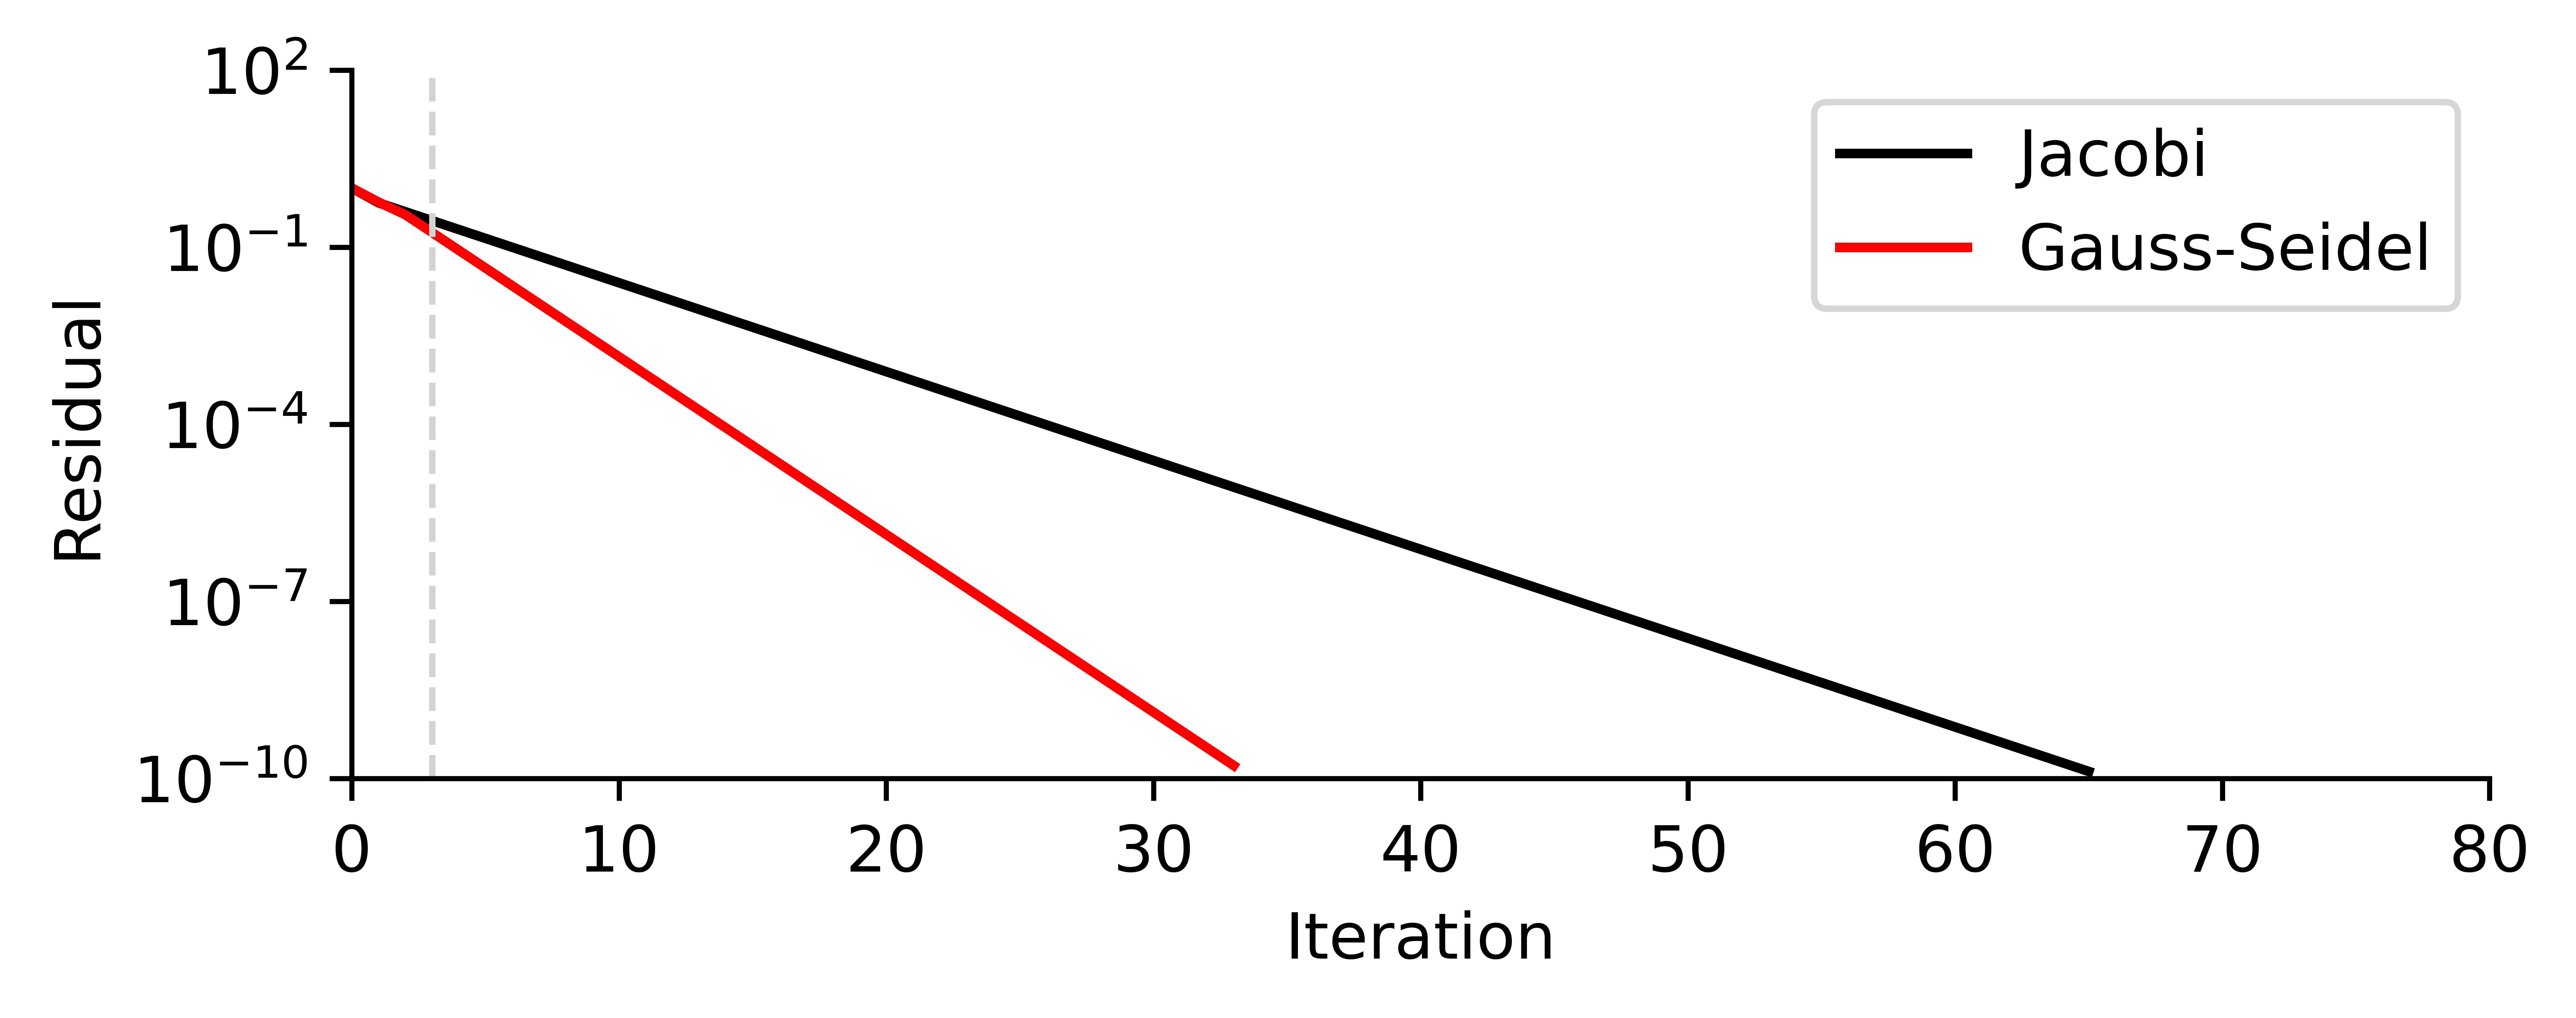
\includegraphics[width=\textwidth]{motivating_example}
    \vspace{-2cm}
  }
}

\begin{frame}
  \centering
  \textbf{Weighted Jacobi iteration}
  \medskip
  \Large
  \[
  \bm{u}_{k+1} = \left( \bm{I} - \omega \bm{D}^{-1} \bm{A} \right) \bm{u}_k
  \]

  \vspace{-1.5cm}
\end{frame}

\begin{frame}
  \centering
  For $\bm{A} \in S_{++}(n)$, \(\omega_{\textrm{opt}} = \dfrac{2}{\lambda_{\min} (\bm{D}^{-1} \bm{A}) + \lambda_{\max} (\bm{D}^{-1} \bm{A})}\)

  \vspace{-1.5cm}
\end{frame}

\begin{frame}
  If we let $\omega$ varies at each iteration $k$, then the system can be solved in exactly 3 iterations provided
  %
  \begin{overprint}
    \onslide<1>
    \[
    \prod_{k=1}^3 \left( \bm{I} - \omega_k \bm{D}^{-1} \bm{A} \right) = \bm{0},
    \]

    \onslide<2>
    \[
    \prod_{k=1}^3 \left( 1 - \omega_k \lambda_k \right) = 0,
    \]
  \end{overprint}

  \medskip

  i.e. $\omega_k$ are the root of this cubic polynomial.

  \vspace{-1cm}
\end{frame}

\begin{frame}
  \begin{overprint}
    \onslide<1>
    \Large
    \[
    \omega_1 = \dfrac{2 + \sqrt{2}}{2}, \quad \omega_2 = 1 \quad \text{and} \quad \omega_3 = \dfrac{2 - \sqrt{2}}{2}
    \]

    \onslide<2>
    \Large
    \[
    {\color{lime} \underbrace{\omega_1 = \dfrac{2 + \sqrt{2}}{2}}_{\textbf{Over-relaxation}}}, \quad \omega_2 = 1 \quad \text{and} \quad \omega_3 = \dfrac{2 - \sqrt{2}}{2}
    \]

    \onslide<3>
    \Large
    \[
    \underbrace{\omega_1 = \dfrac{2 + \sqrt{2}}{2}}_{\textbf{Over-relaxation}}, \quad \omega_2 = 1 \quad \text{and} \quad {\color{red} \underbrace{\omega_3 = \dfrac{2 - \sqrt{2}}{2}}_{\color{red} \textbf{Under-relaxation}}}
    \]

  \end{overprint}

  \vspace{-1cm}
\end{frame}

\begin{frame}
  \begin{minipage}{.48\textwidth}
    Neat example proposed by a Master student in Stanford back in 2014.
    Since then, Jacobi has seen more than 1000x speed-up!
    \vspace{-1cm}
  \end{minipage}%
  \hfill
  \begin{minipage}{.48\textwidth}
    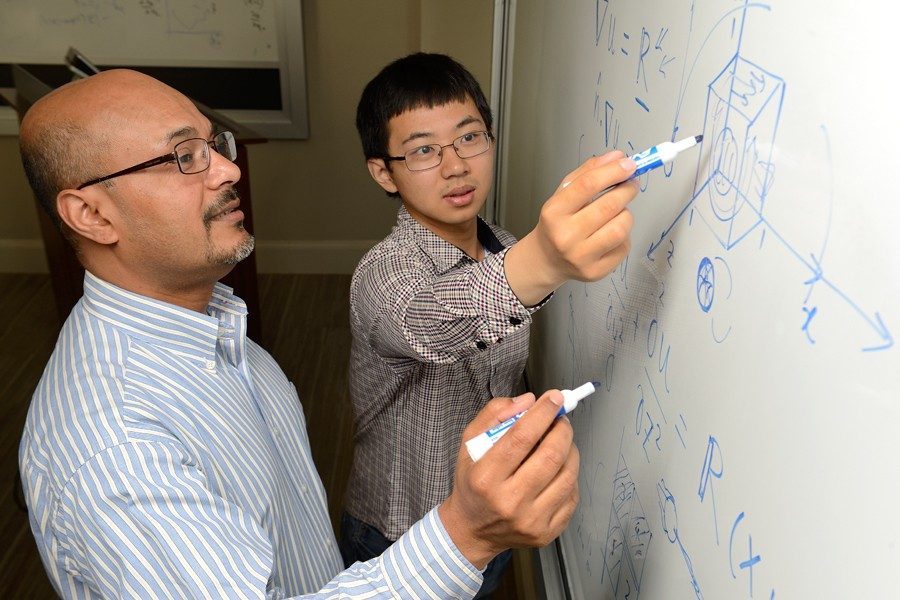
\includegraphics[width=\textwidth]{yang_mittal}
  \end{minipage}
\end{frame}


{
  \setbeamercolor{background canvas}{bg=white}
  \frame{
    \vfill
    \centering
        {\Large
          {\color{black} \textbf{Scheduled-Relaxation Jacobi}}
        }

        \medskip

        {\large
          {\color{gray} \textbf{Fast! Faster! Fastest!}}
        }
        \vfill
  }
}

\begin{frame}
  \alert{\textbf{Major problem :}} In the general high-dimensional case, computing the optimal sequence $\omega_k$ is not feasible.
  It relies on the eigenvalues $\lambda_k$ requiring $\mathcal{O}(n^3)$ operations.
  
  \vspace{-1.5cm}
\end{frame}

\begin{frame}
  \alert{\textbf{Luck :}} If $\bm{A}$ results from the discretization of an elliptic partial differential equation, Adsuara \emph{et al.} provide an easy way to compute the optimal set of weights $\omega_k$.
  
  \vspace{-1.5cm}
\end{frame}

\begin{frame}
  \begin{overprint}
    \onslide<1>
    \[
    \bm{e}_{k+1} = \left( \bm{I} - \omega \bm{D}^{-1} \bm{A} \right) \bm{e}_k
    \]

    \onslide<2>
    \[
    e_j^{(k+1)} = e_j^{(k)} + \dfrac{\omega}{2} \left( e_{j+1}^{(k)} - 2 e_j^{(k)} + e_{j-1}^{(k)} \right)
    \]

    \onslide<3>
    \[
    G(\kappa) = 1 - \omega \kappa \quad \text{with} \quad \kappa = 2 \sin^2\left( \dfrac{q \Delta x}{2} \right)
    \]

    \onslide<4>
    \[
    G_M(\kappa) = \prod_{i=1}^M \left( 1 - \omega \kappa \right)
    \]

    \onslide<5>
    \[
    \omega_k = 2 \left( \kappa_{\max} + \kappa_{\min} - (\kappa_{\max} - \kappa_{\min}) \cos \left( \pi \dfrac{2k-1}{2M} \right) \right)^{-1}
    \]
  \end{overprint}
  \vspace{-1cm}
\end{frame}

{
  \setbeamercolor{background canvas}{bg=white}
  \begin{frame}[fragile]{}{}
    \vfill
    \begin{lstlisting}[backgroundcolor=\color{white}, basicstyle=\ttfamily\footnotesize\color{black}]
      import numpy as np
      
      def scheduled_relaxation_jacobi(A, b, x, w, maxiter, tol):
      
          # --> Extrait la diagonale de A.
          invD = 1.0 / np.diag(A)
          n = len(w)
          
          # --> Iteration de Jacobi.
          for k in range(maxiter):
              r = b - A @ x
              if np.linalg.norm(r) < tol:
                  break
              x -= w[k % n] * invD * r
        
        return x
    \end{lstlisting}
    \vfill
  \end{frame}
              }

\begin{frame}[t, c]{}{}
  \centering
  \textbf{Benchmark example}
  \medskip
  \large
  \[
  \dfrac{\partial^2 u}{\partial x^2} = 1, \quad x \in \left[0, 1\right], \quad u(0) = u(1) = 0.
  \]
  
  \vspace{-1cm}
\end{frame}

{
  \setbeamercolor{background canvas}{bg=white}
  \begin{frame}
    \begin{overprint}
      \onslide<1>
      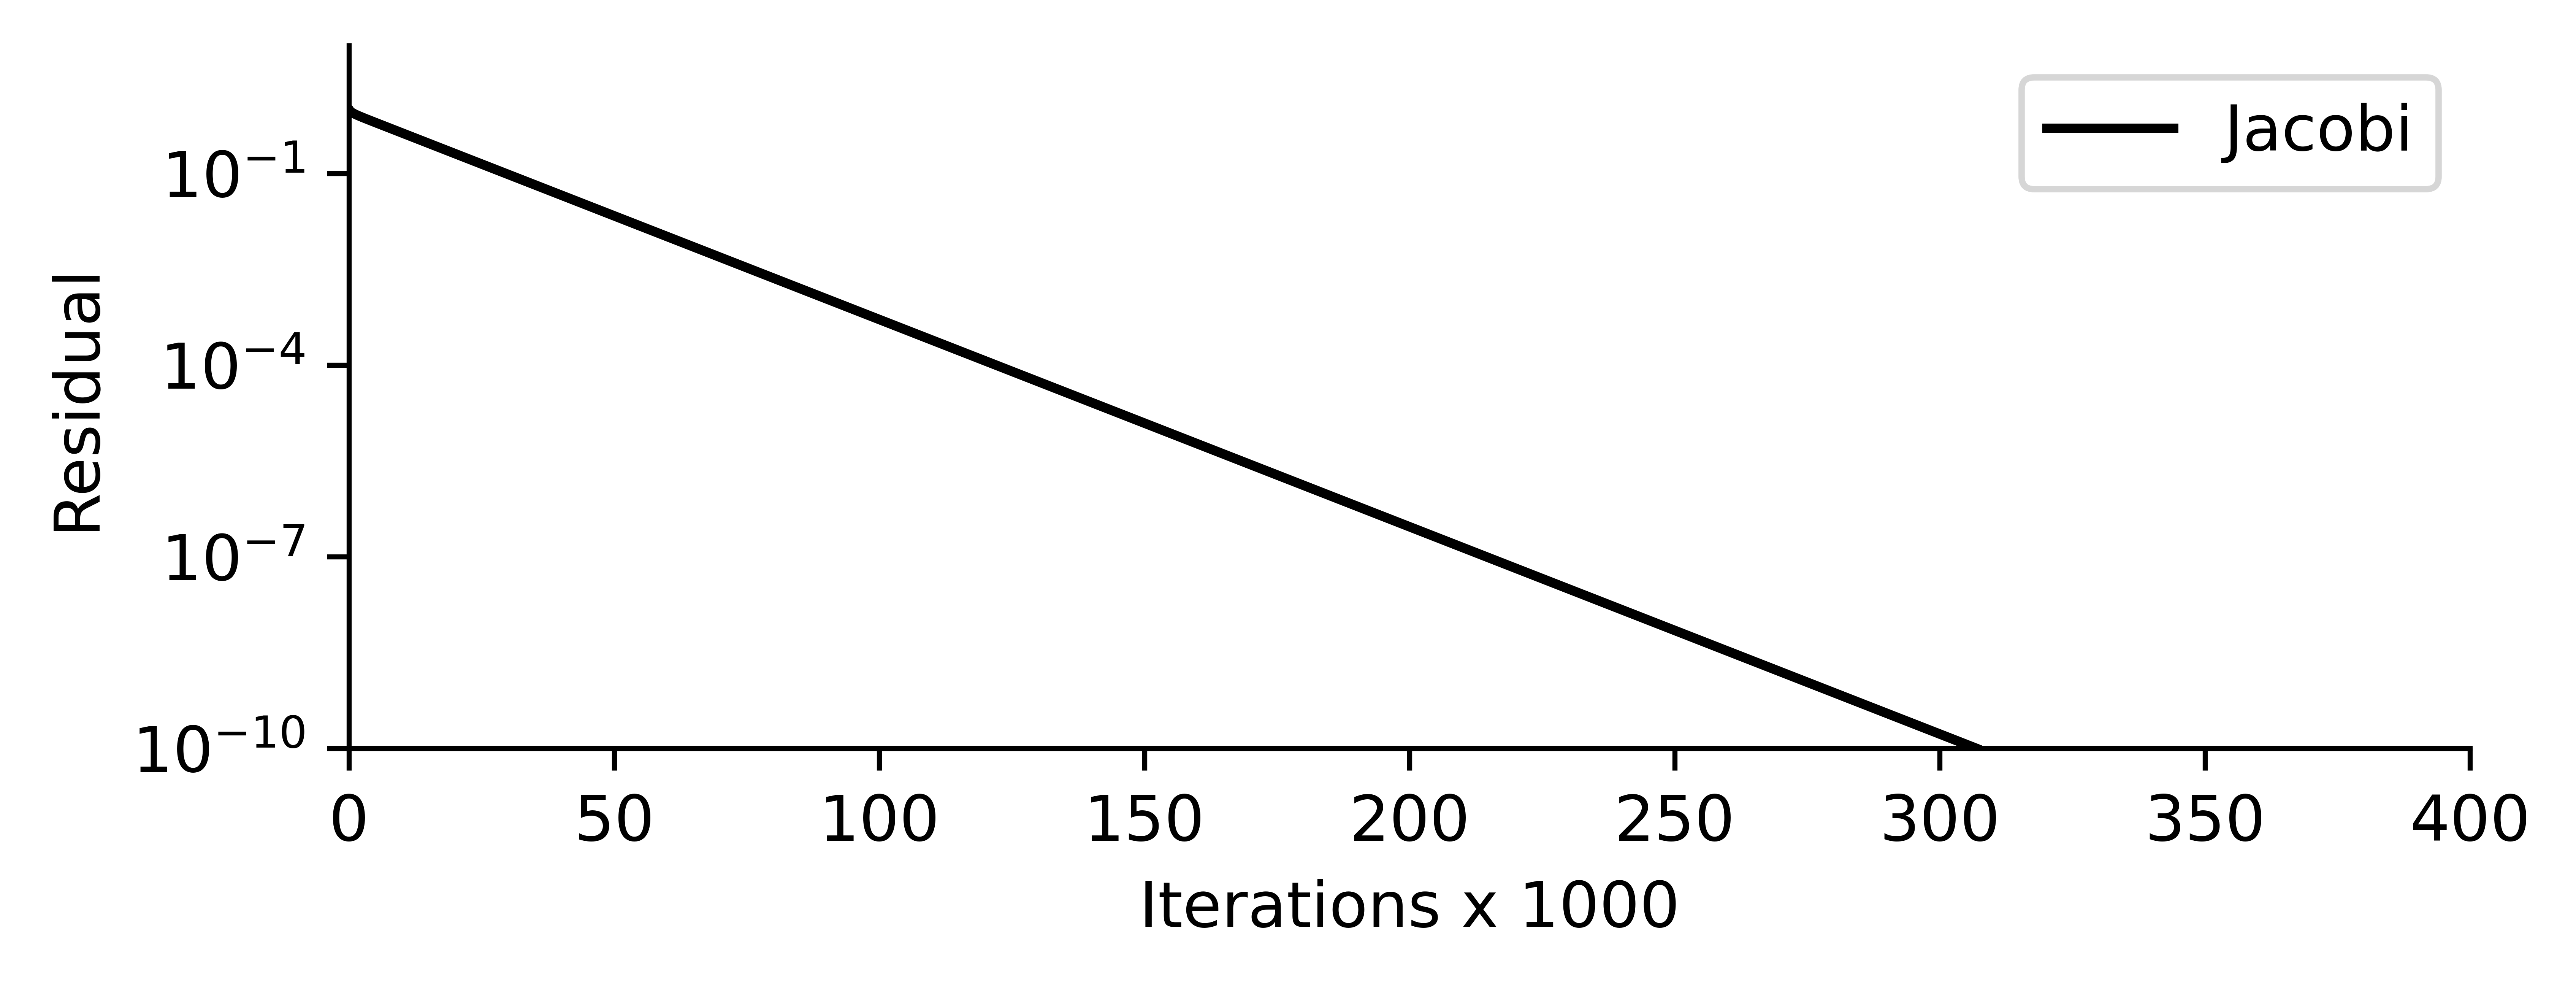
\includegraphics[width=\textwidth]{comparaisons_1D_jacobi}

      \onslide<2>
      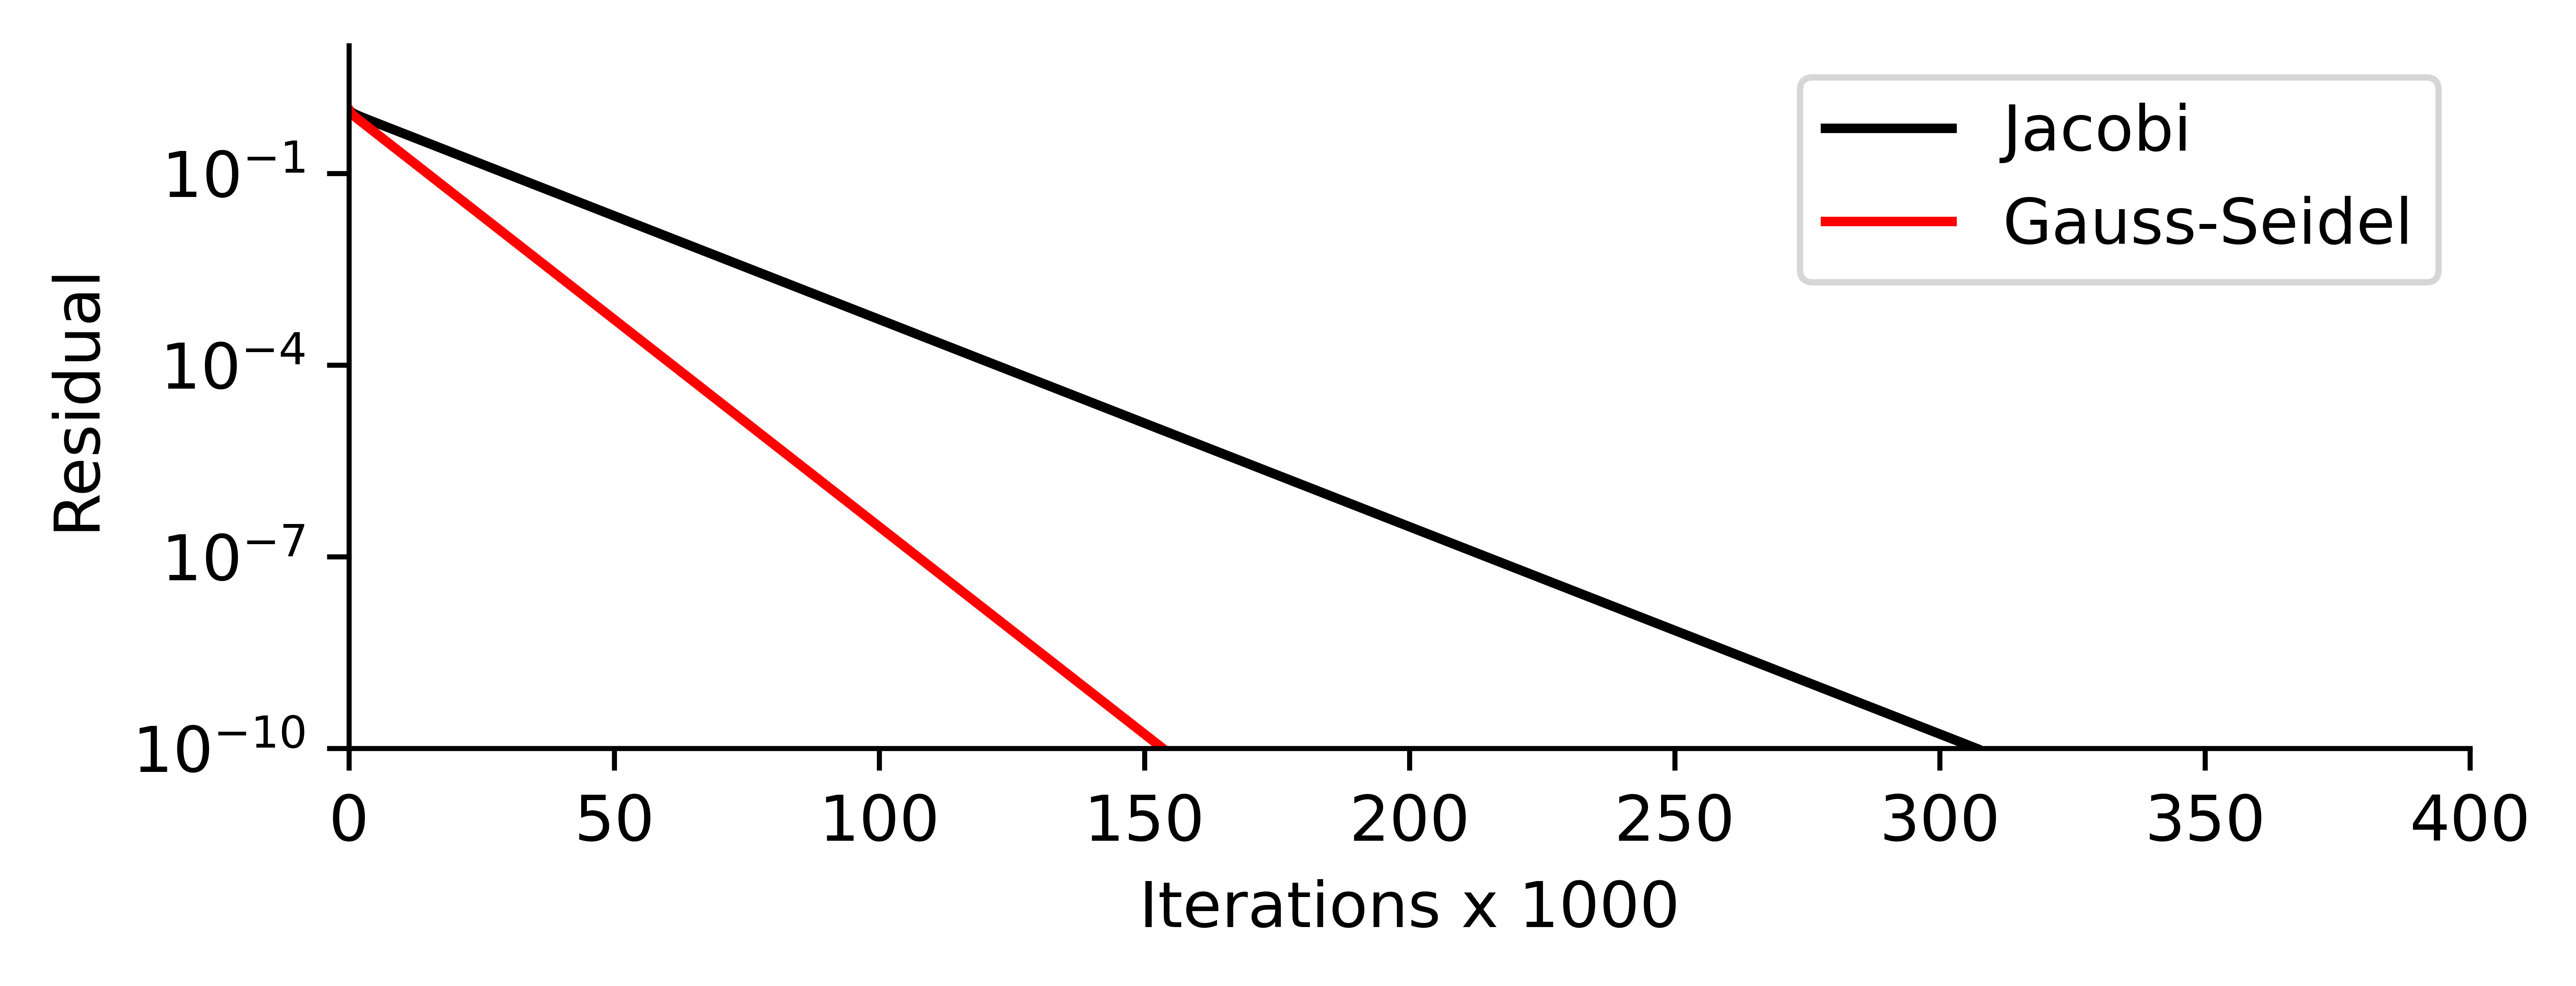
\includegraphics[width=\textwidth]{comparaisons_1D_gs}

      \onslide<3>
      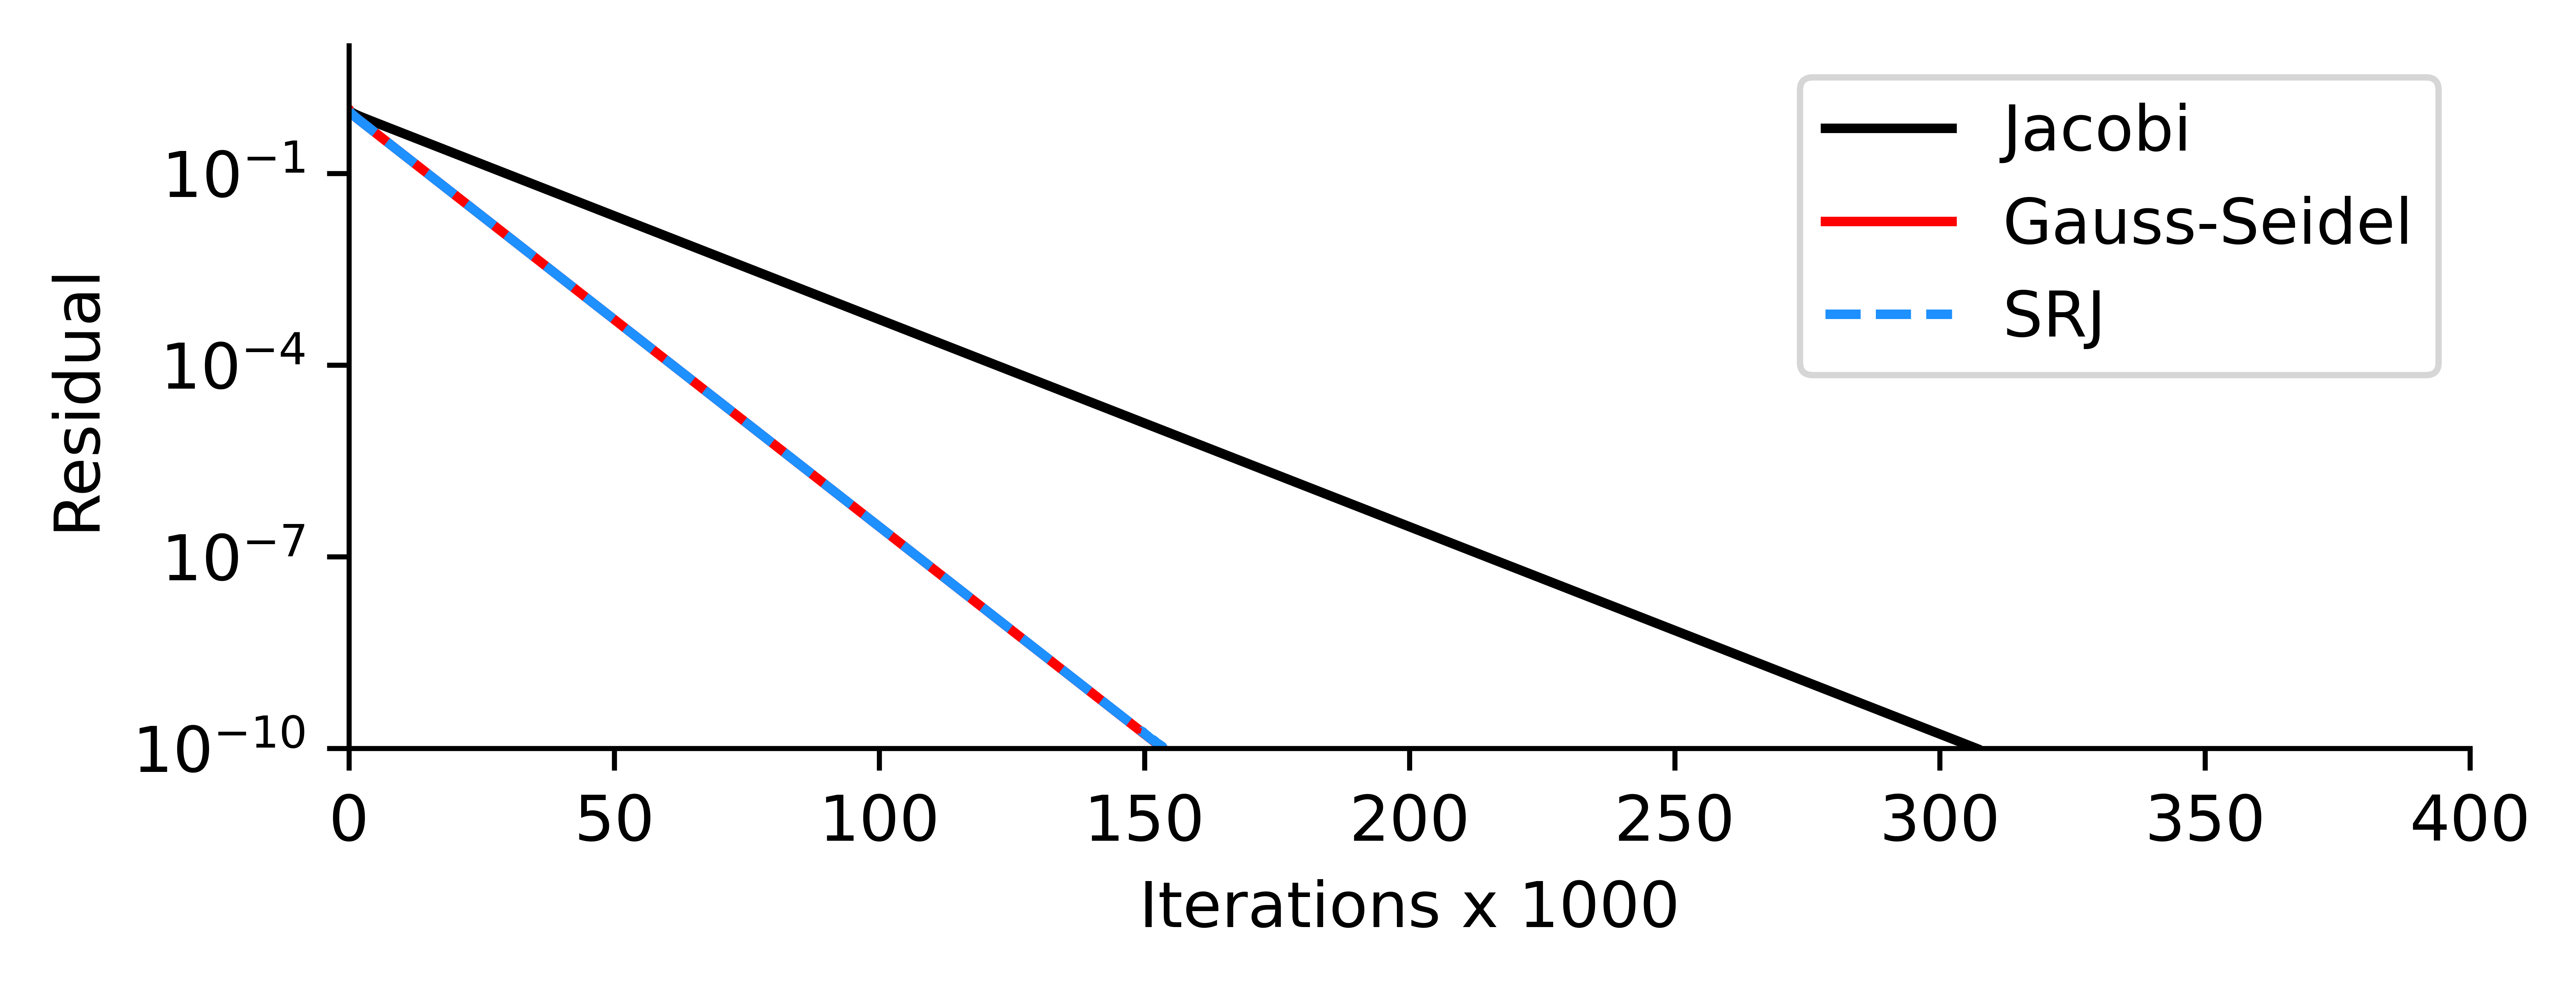
\includegraphics[width=\textwidth]{comparaisons_1D_srj_k=2}

      \onslide<4>
      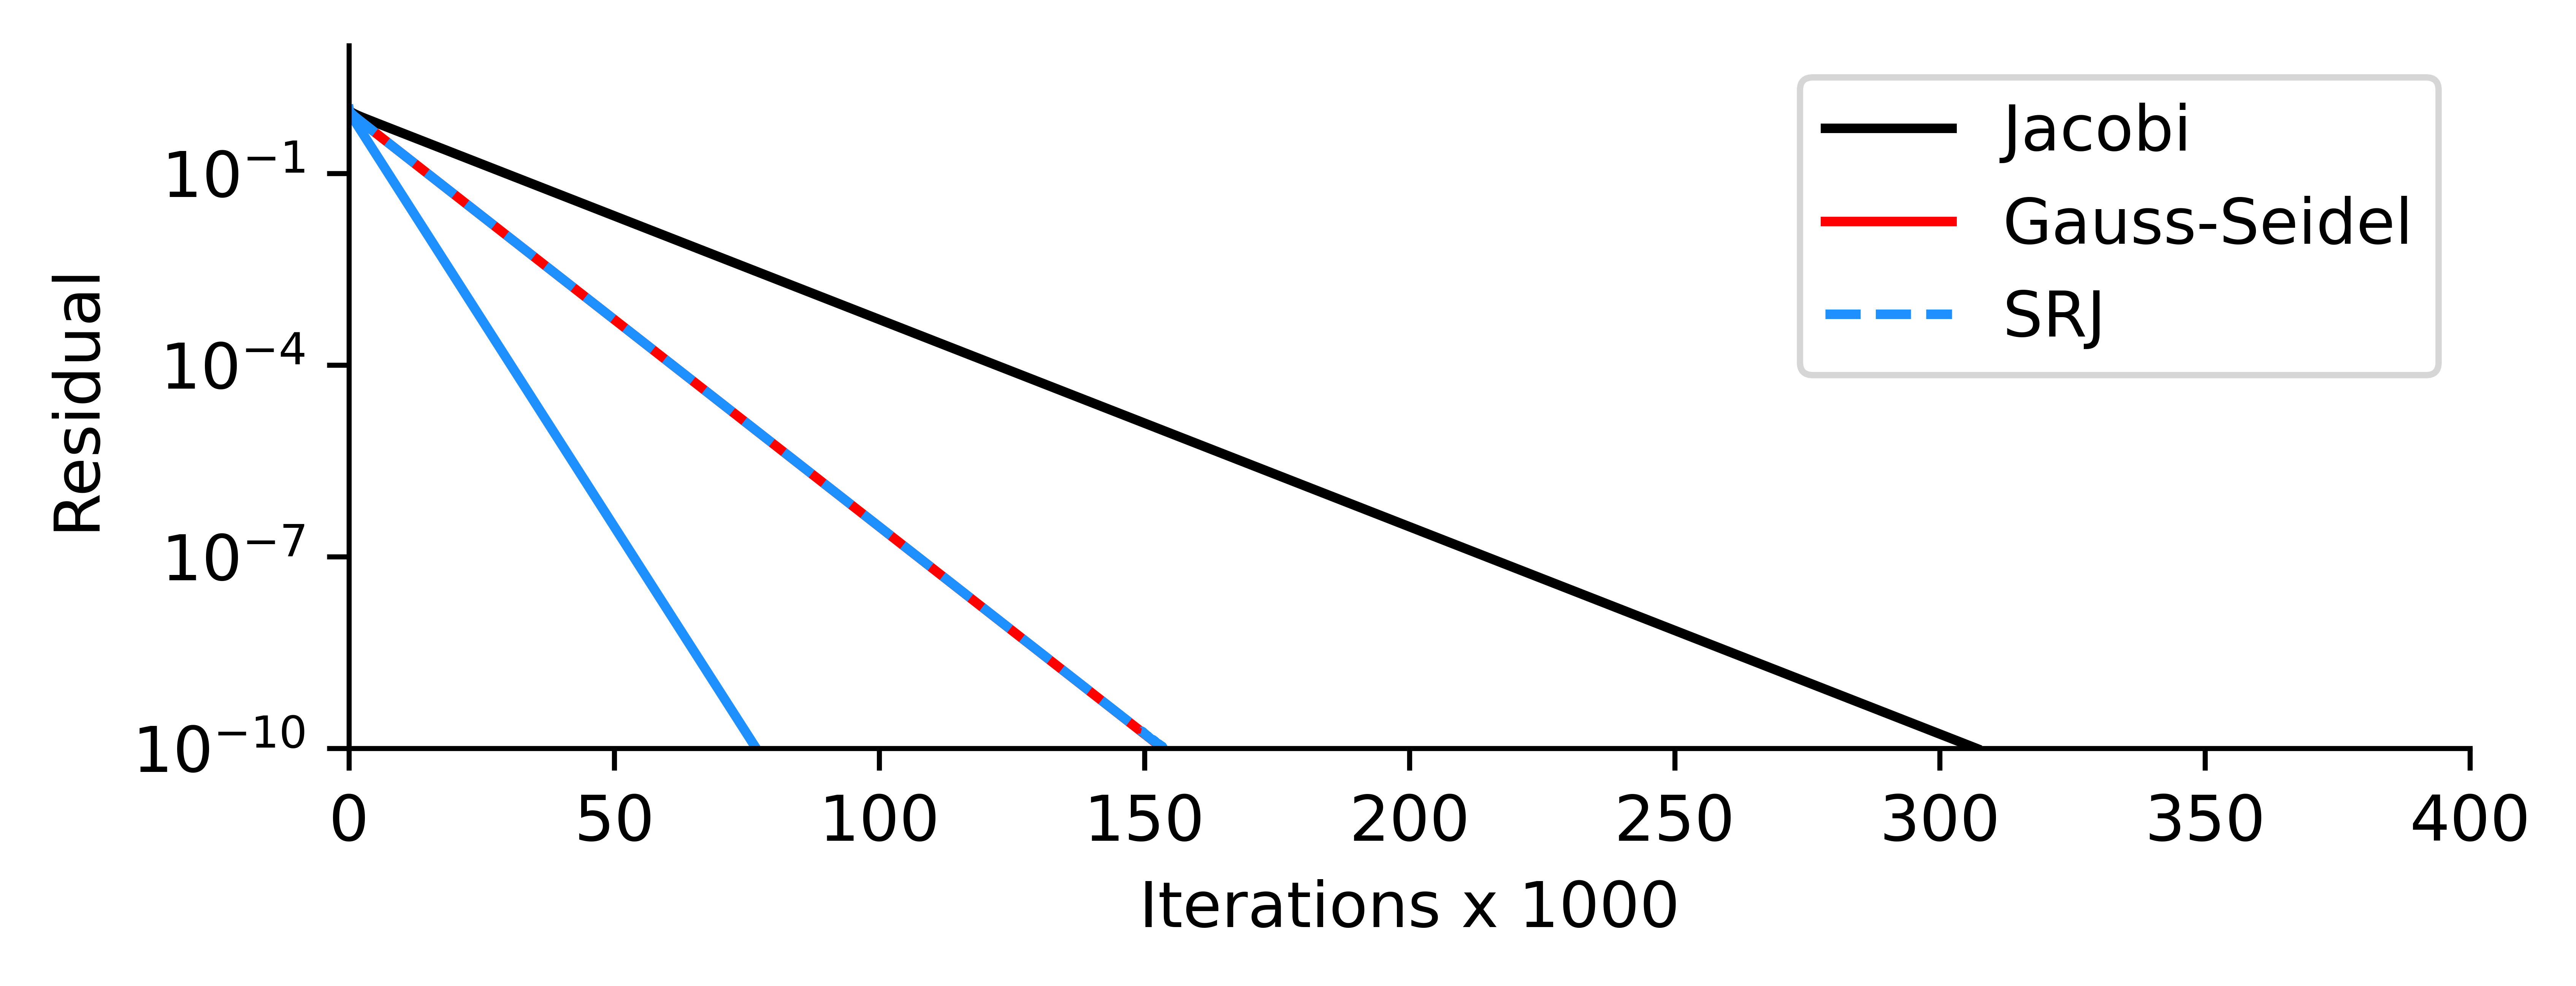
\includegraphics[width=\textwidth]{comparaisons_1D_srj_k=4}

      \onslide<5>
      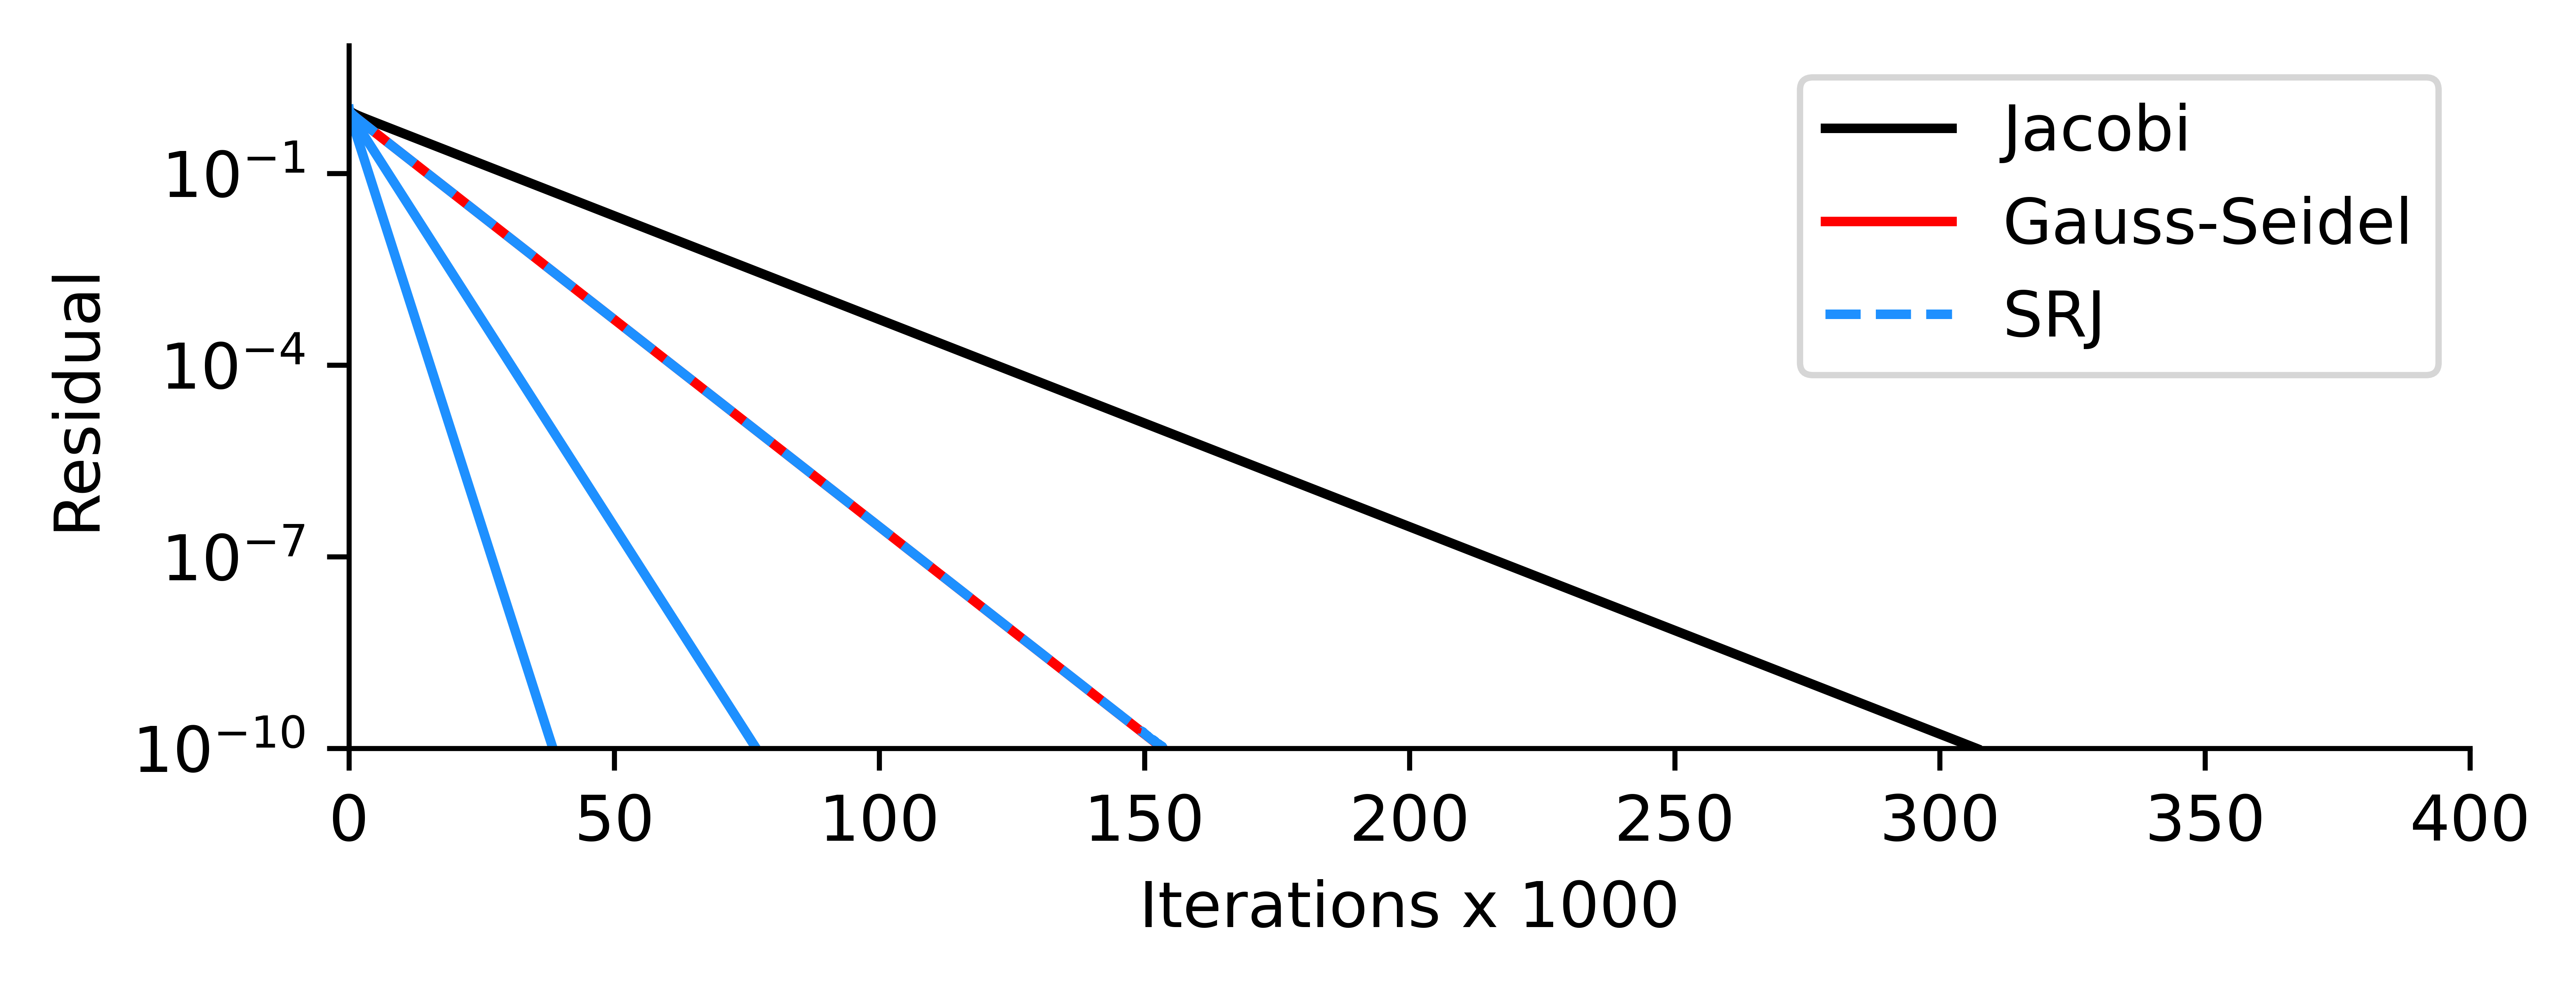
\includegraphics[width=\textwidth]{comparaisons_1D_srj_k=8}

      \onslide<6>
      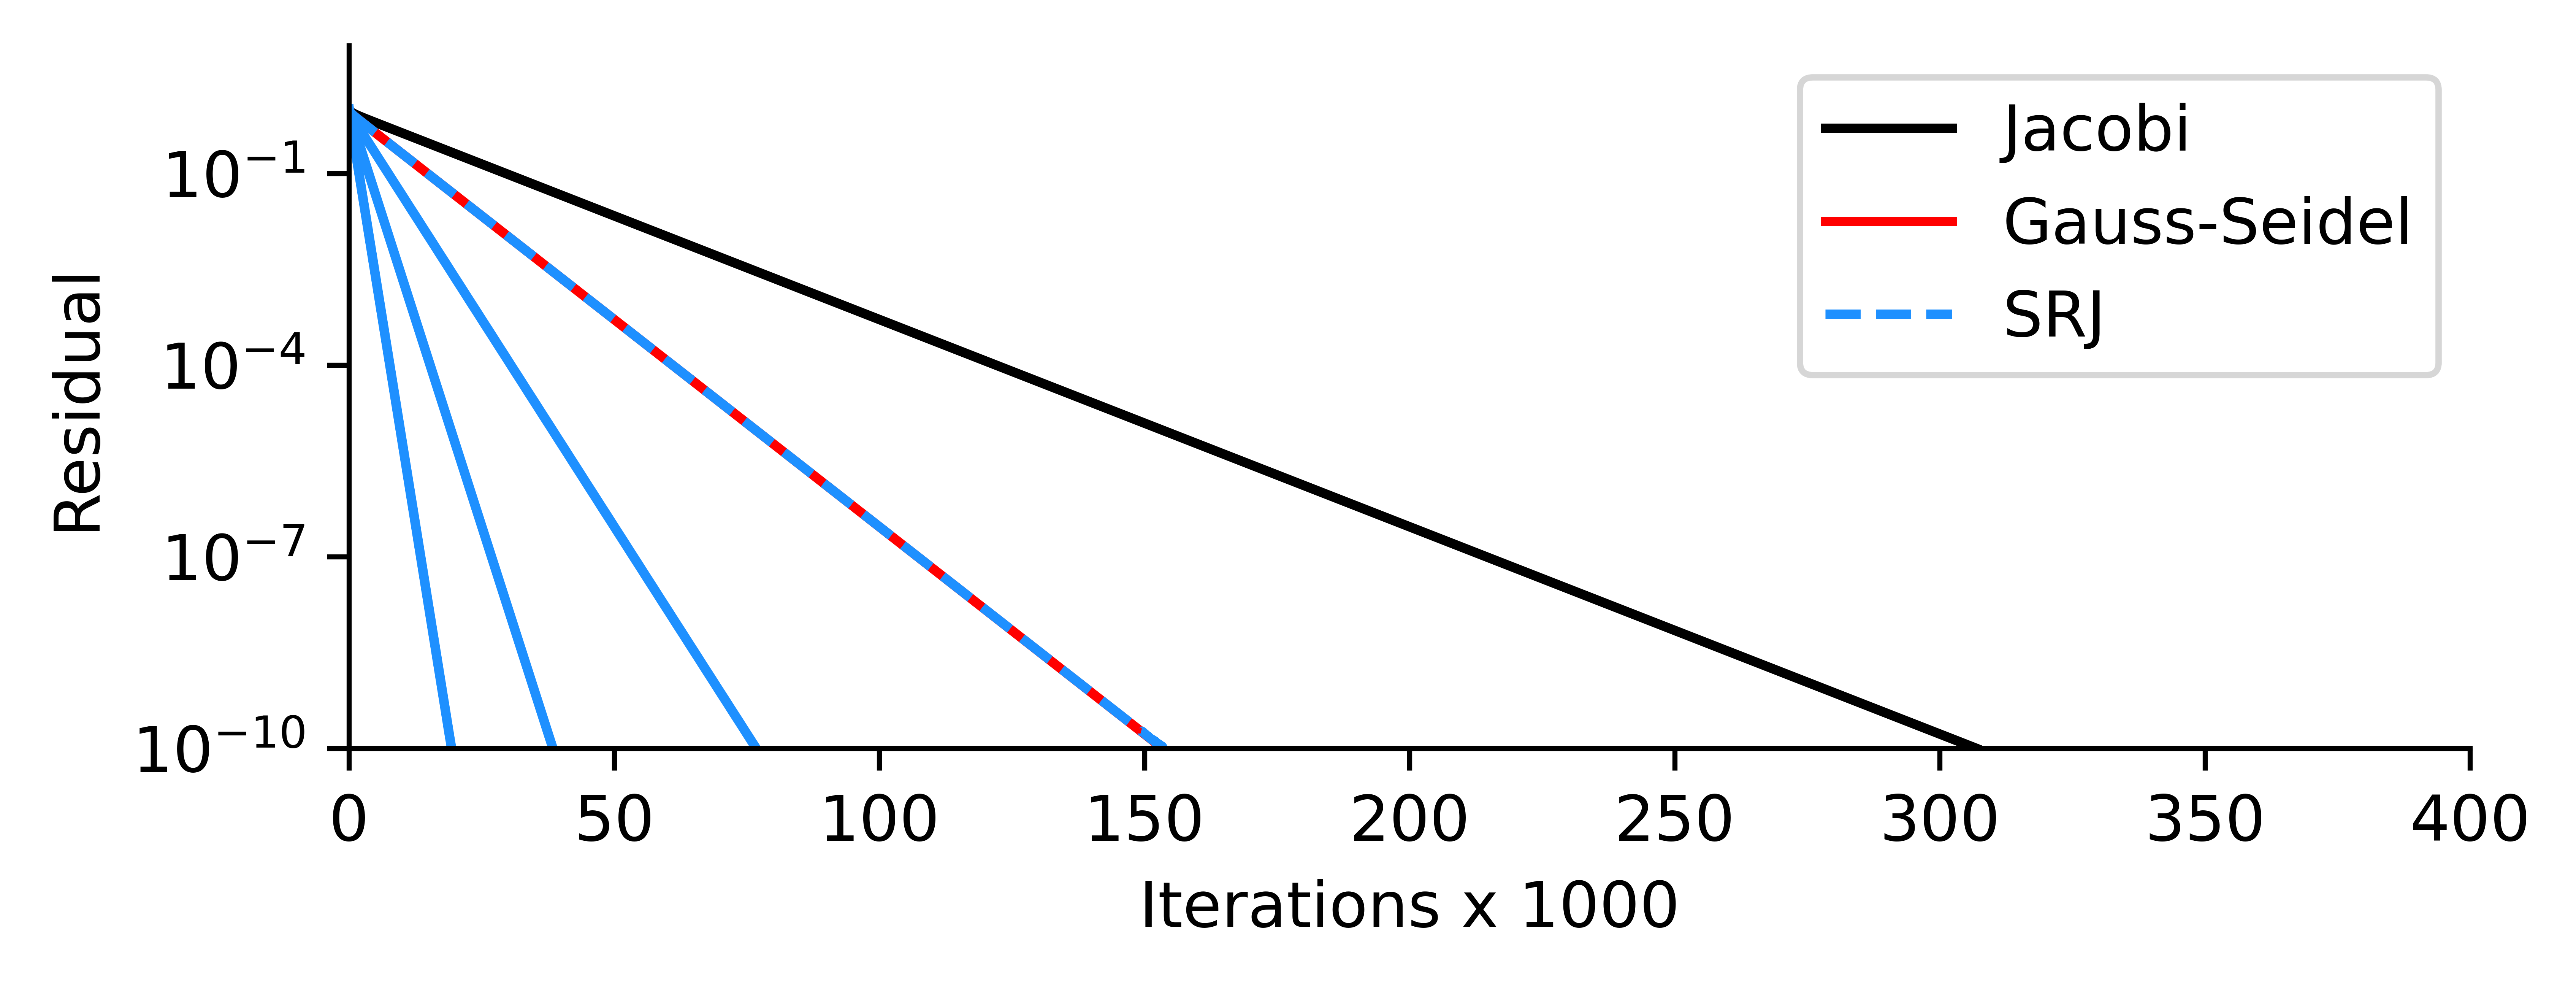
\includegraphics[width=\textwidth]{comparaisons_1D_srj_k=16}

      \onslide<7>
      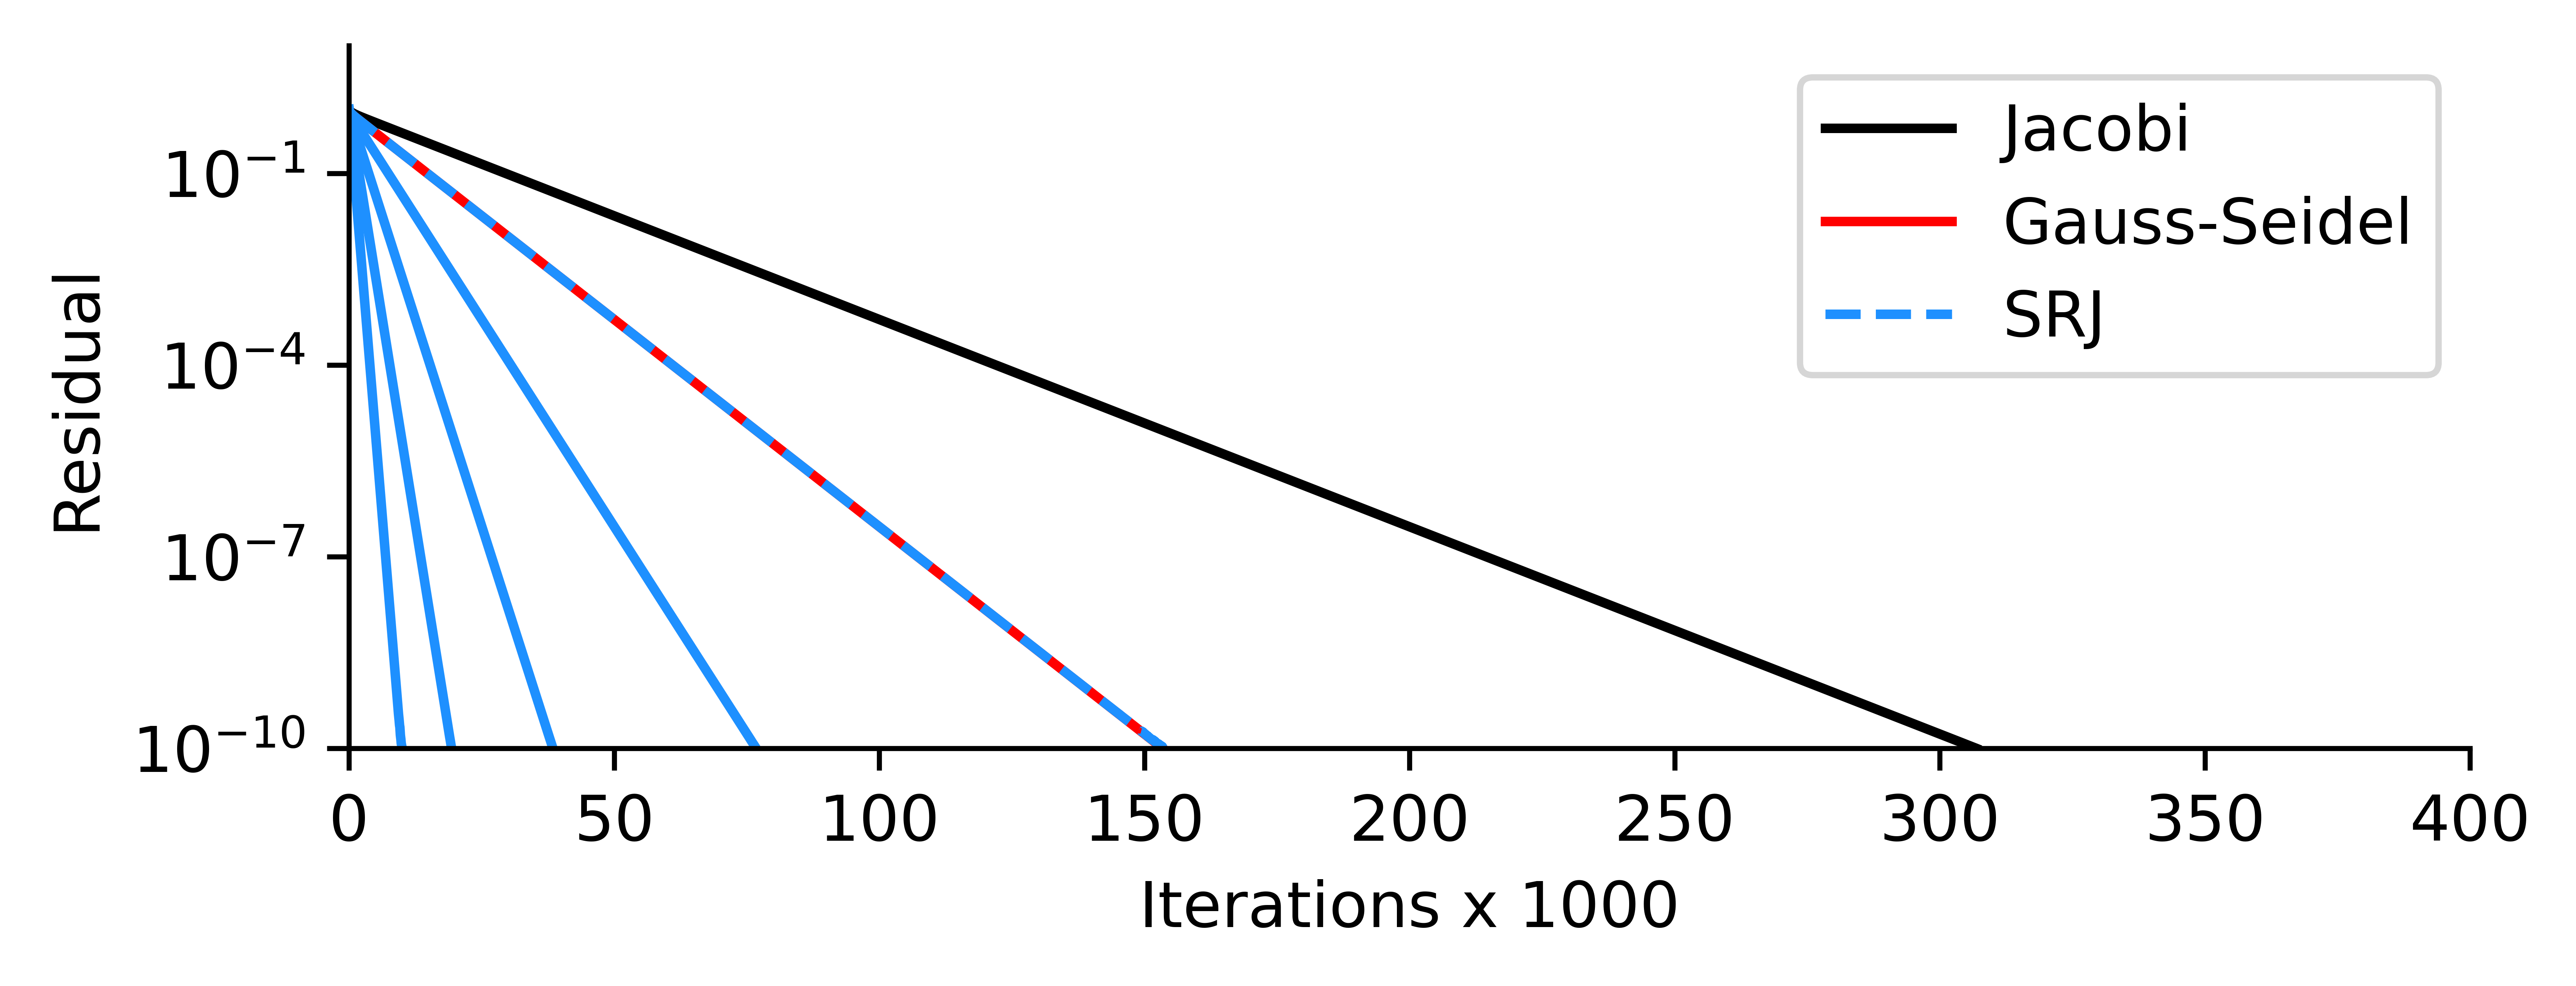
\includegraphics[width=\textwidth]{comparaisons_1D_srj_k=32}

      \onslide<8>
      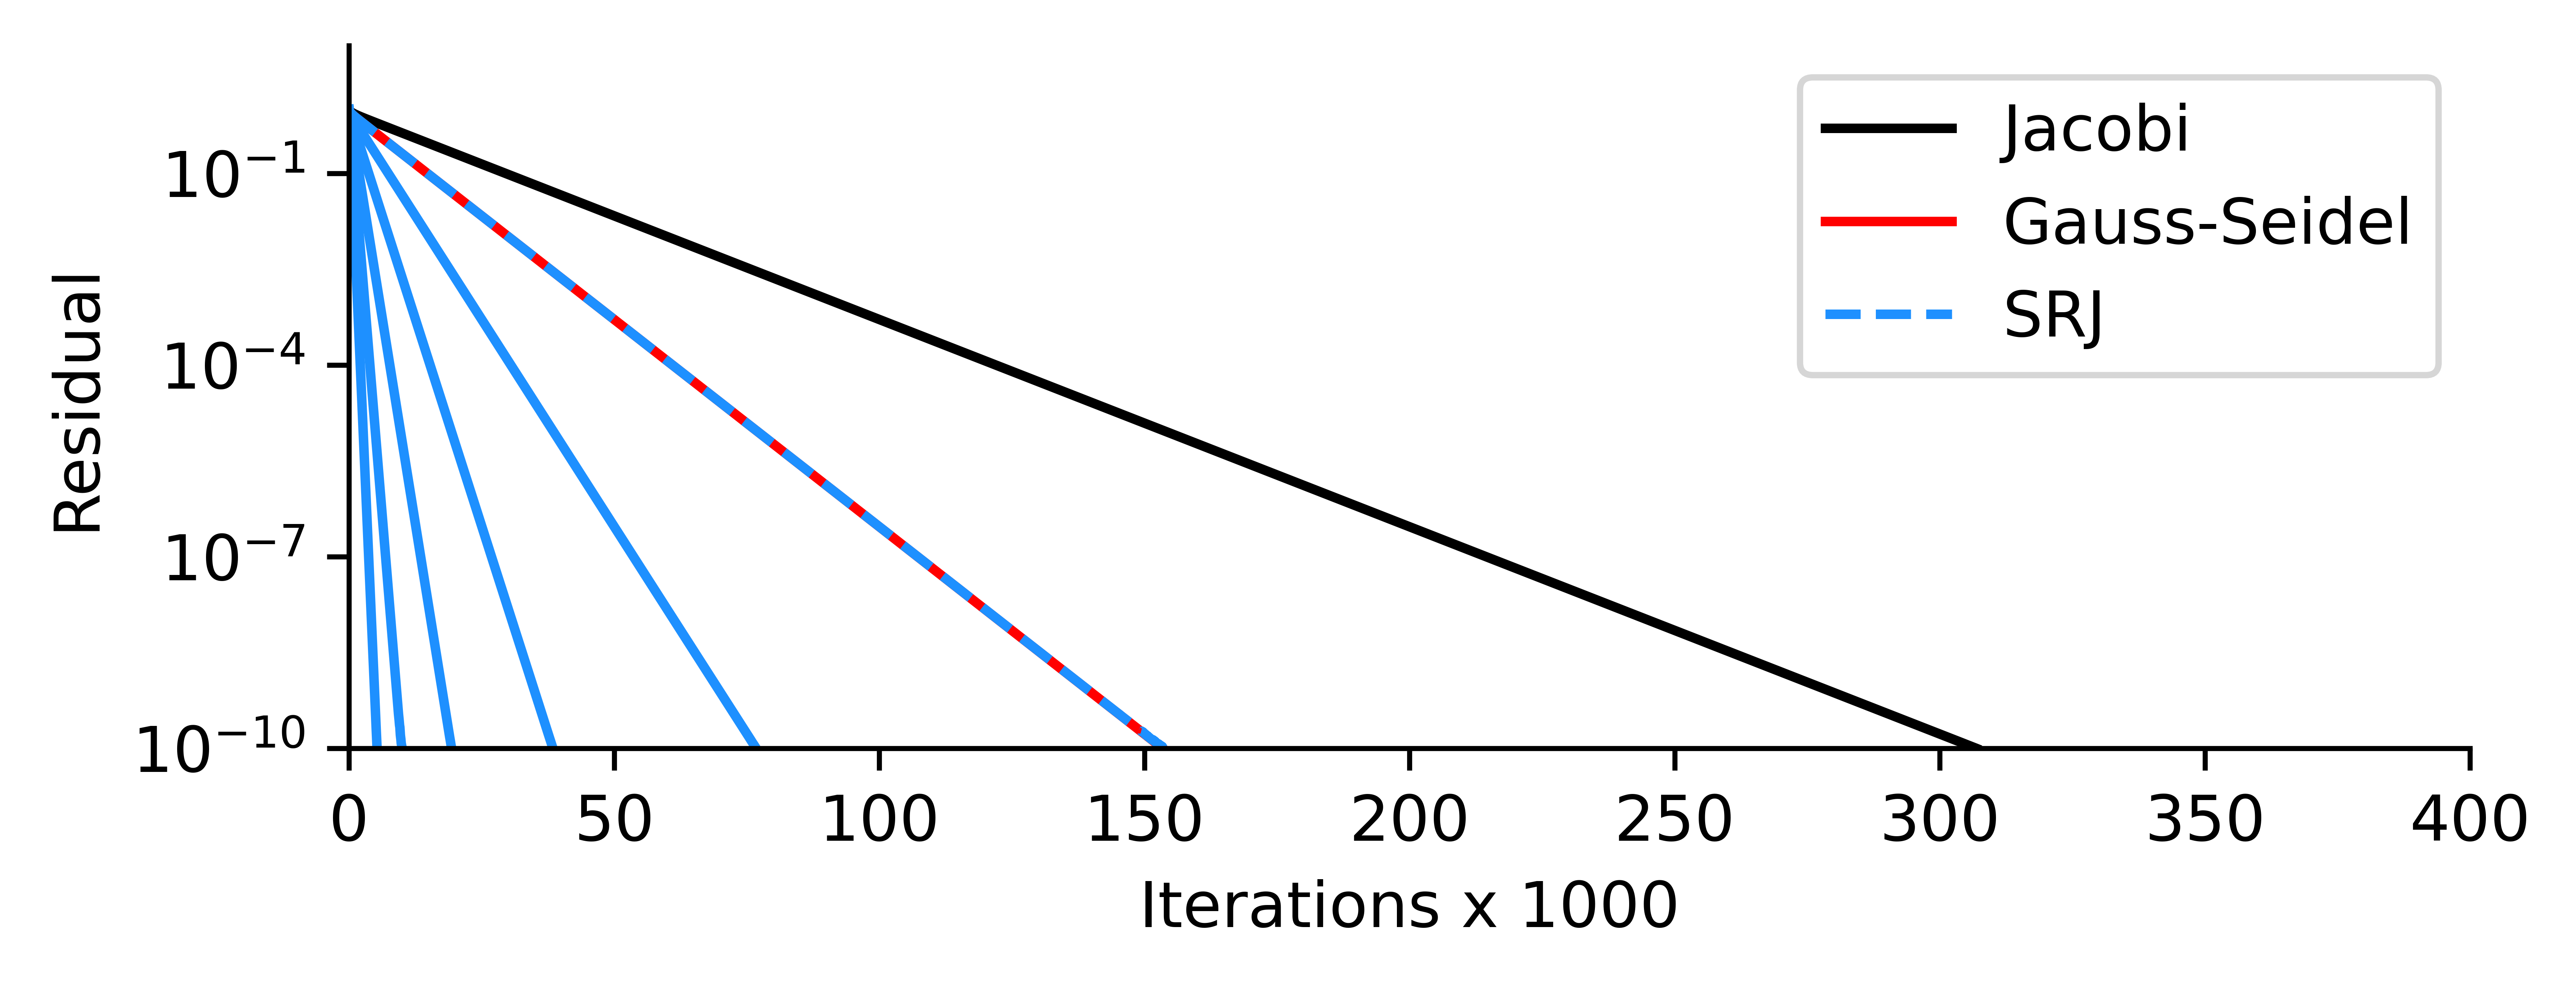
\includegraphics[width=\textwidth]{comparaisons_1D_srj_k=64}

      \onslide<9>
      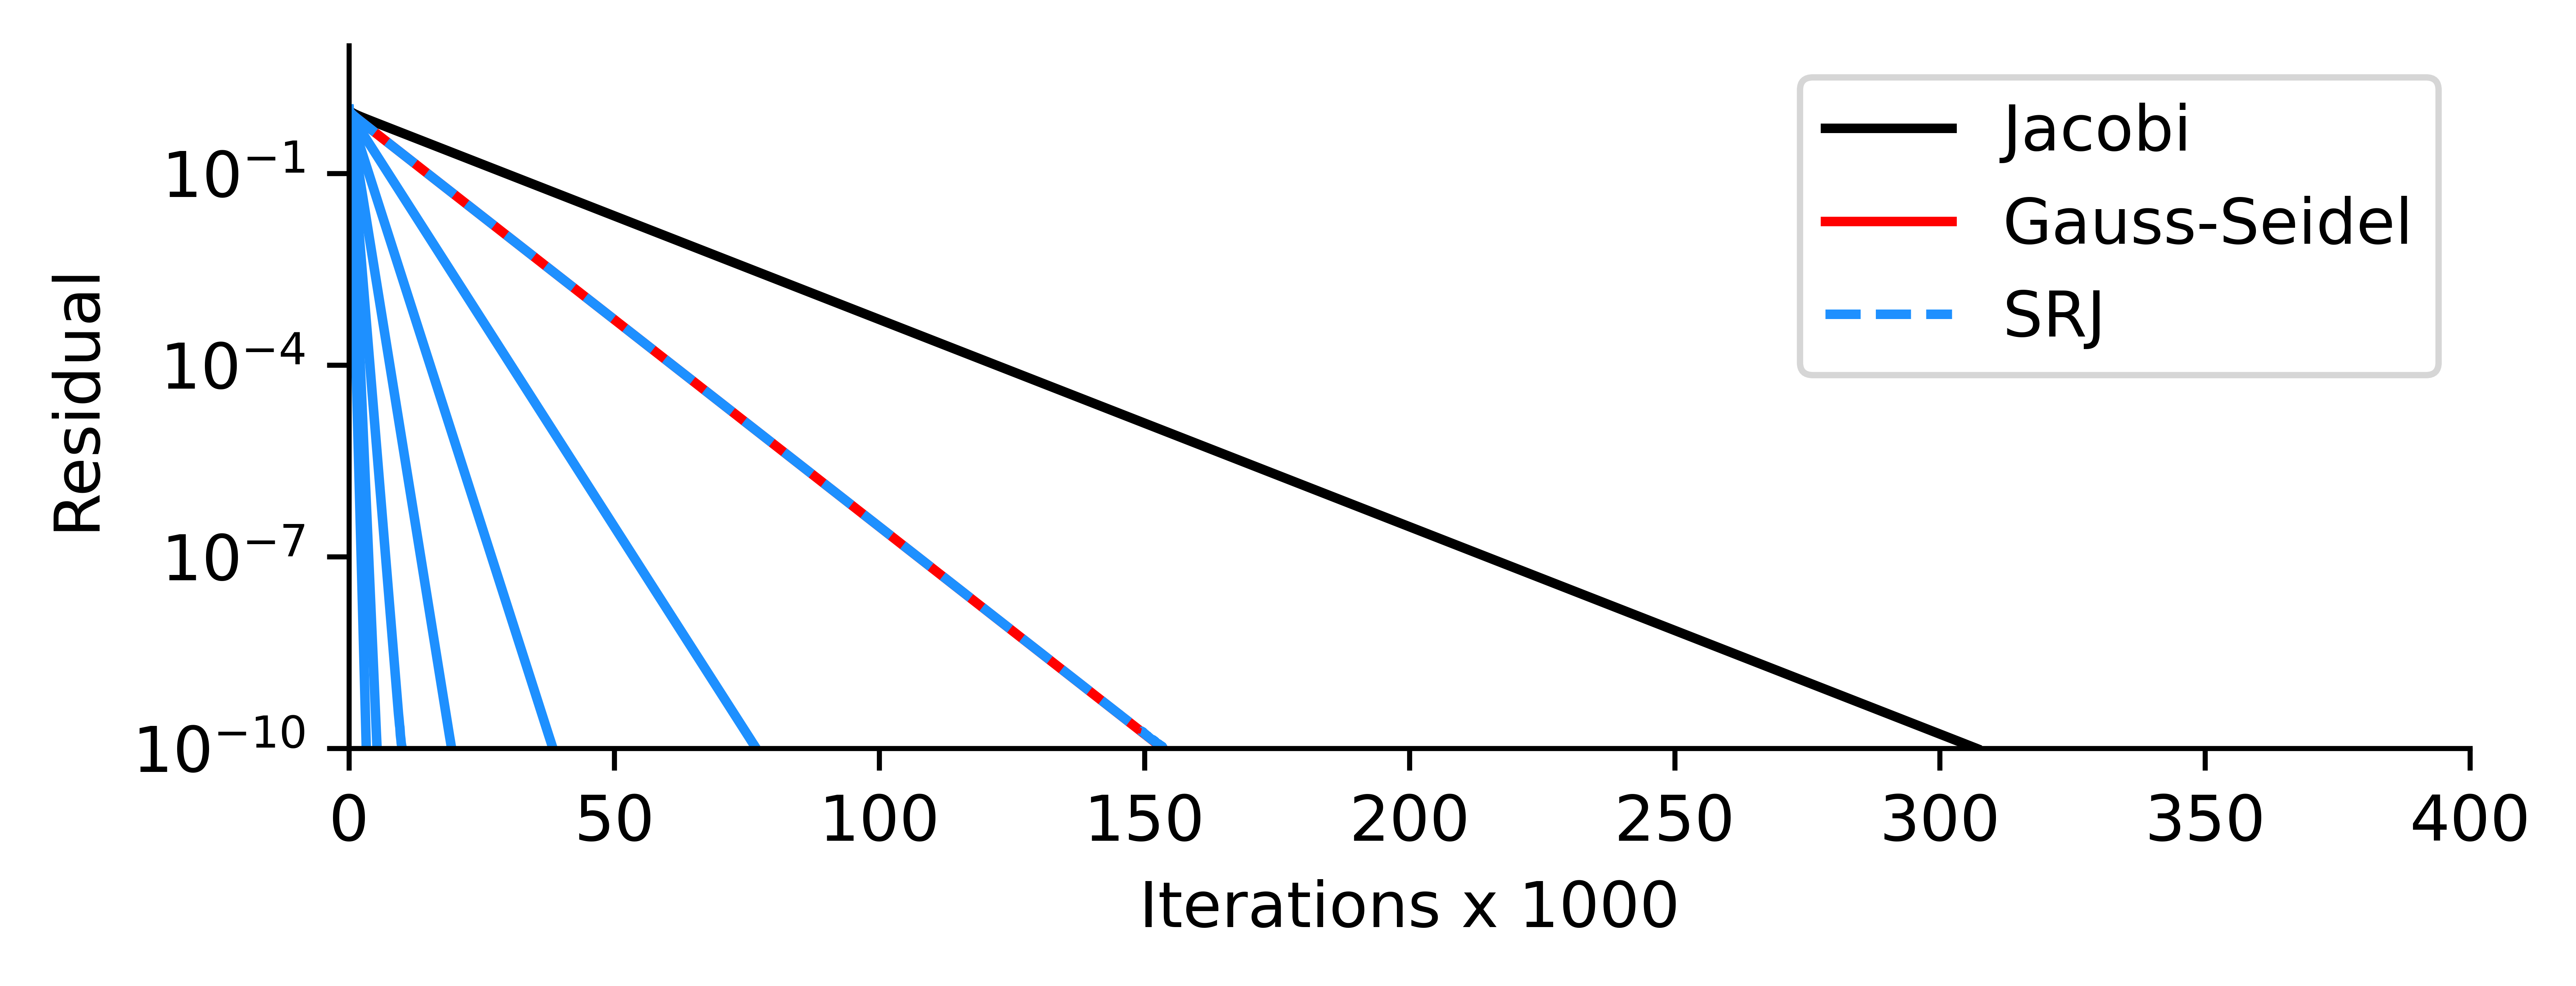
\includegraphics[width=\textwidth]{comparaisons_1D_srj_k=128}

      \onslide<10>
      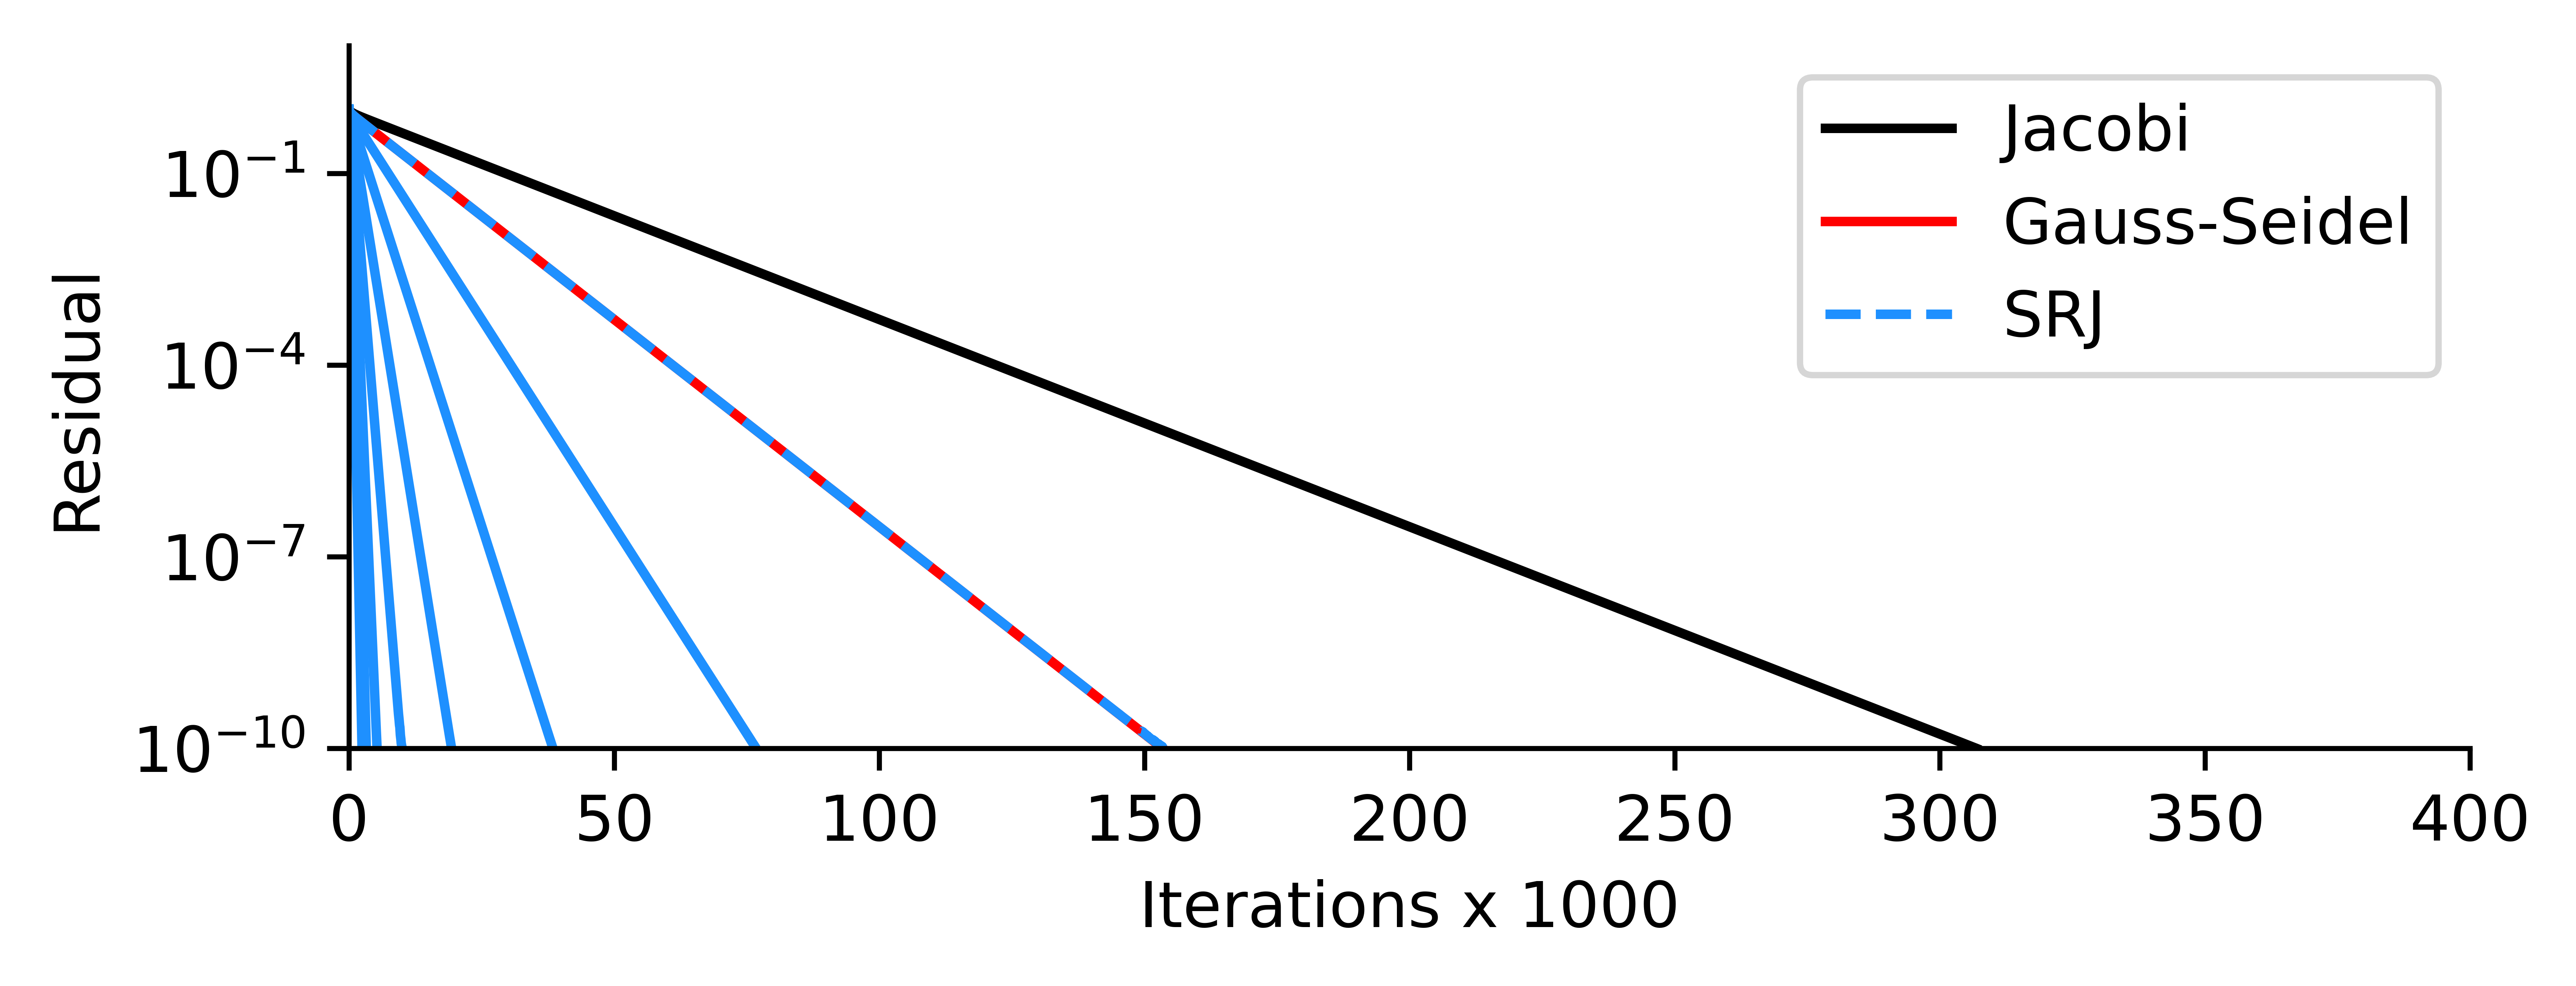
\includegraphics[width=\textwidth]{comparaisons_1D_srj_k=256}

      \onslide<11>
      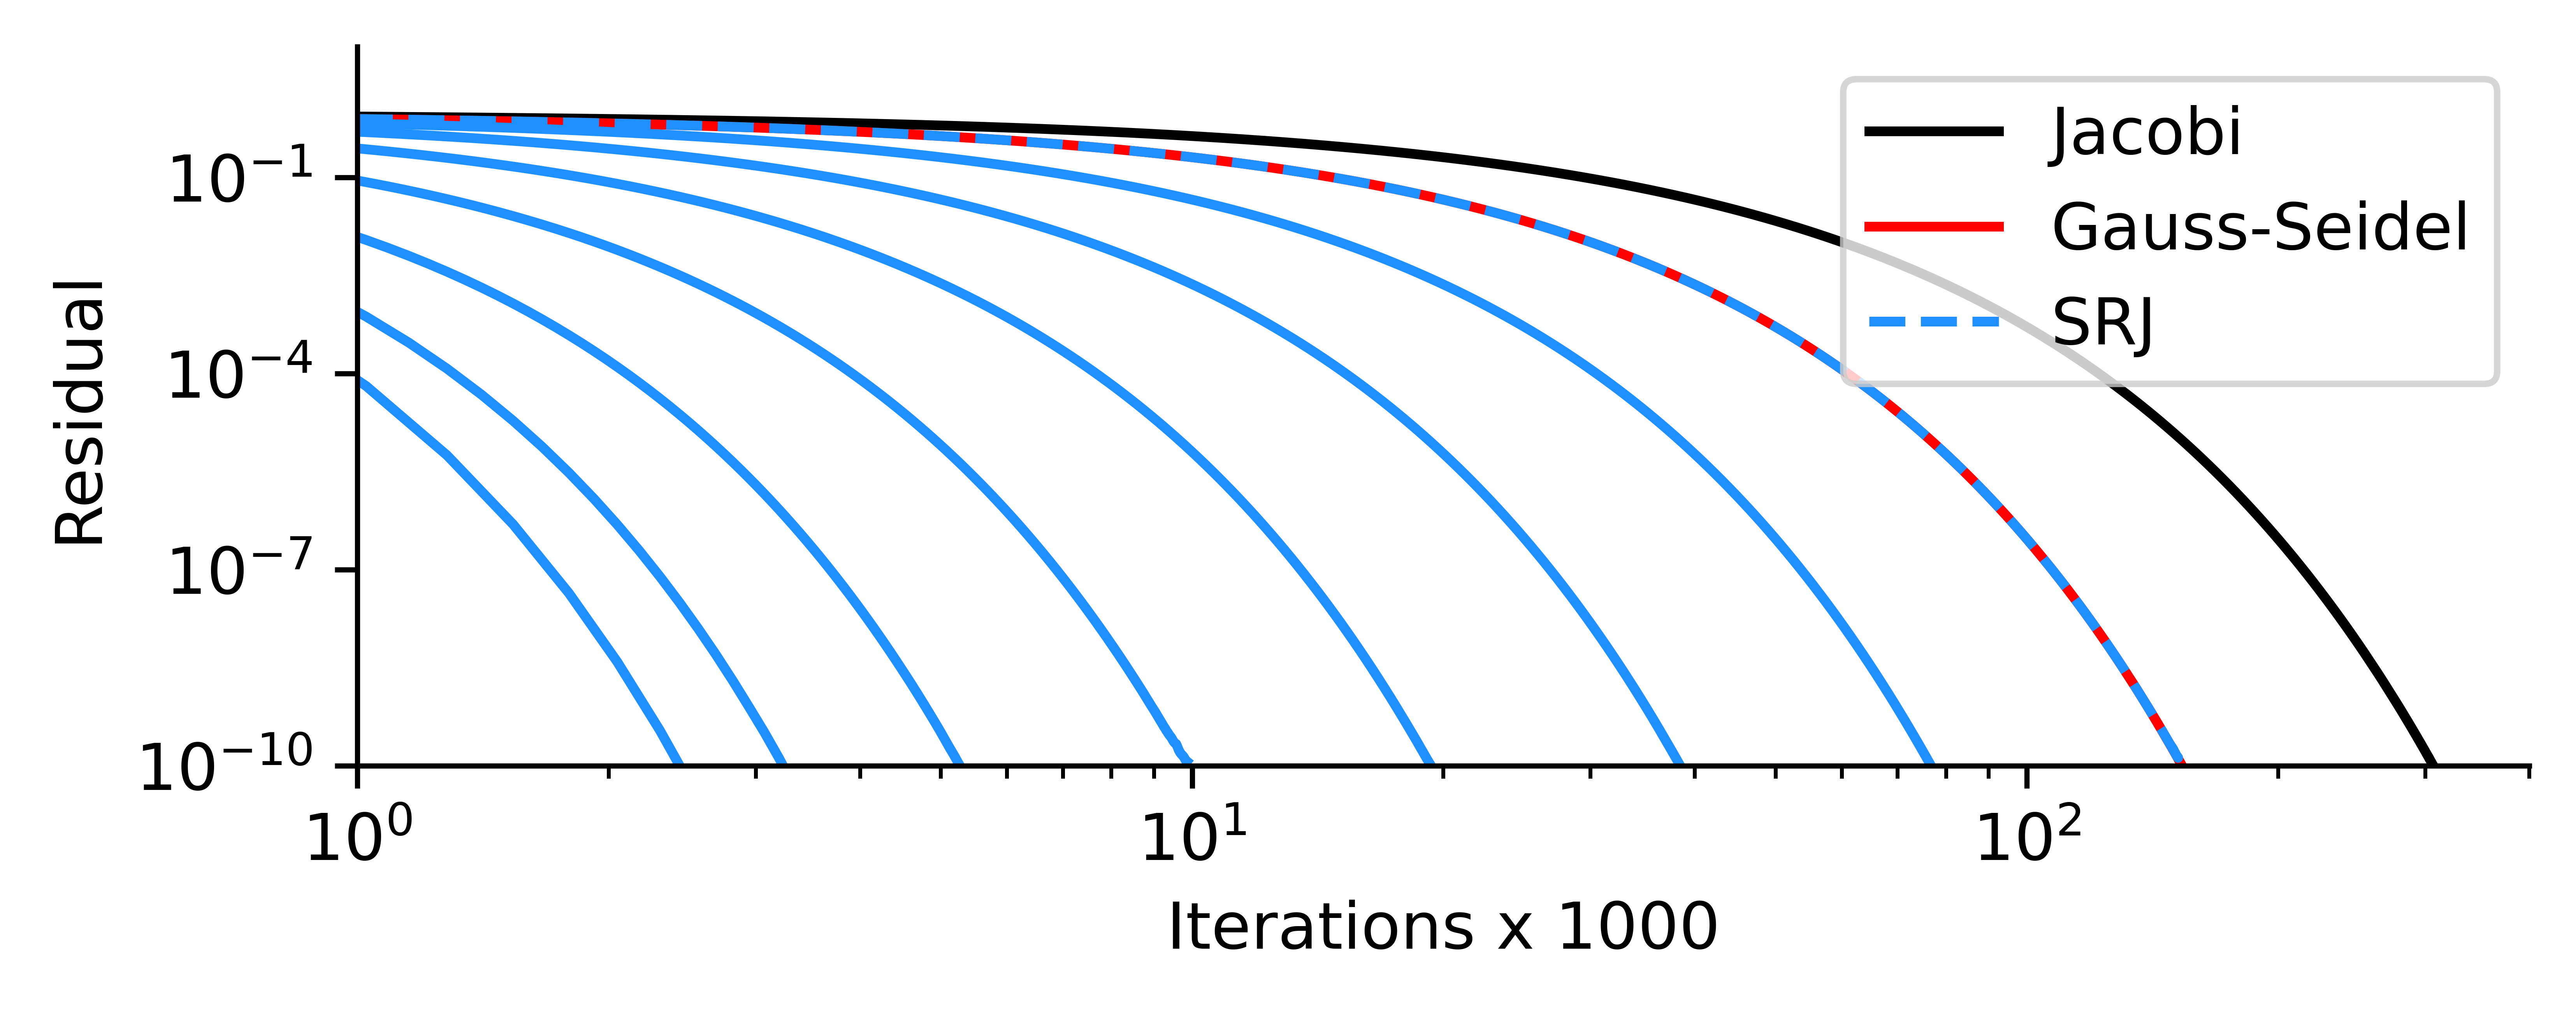
\includegraphics[width=\textwidth]{comparaisons_1D_logscale}

    \end{overprint}
    \vspace{-2cm}
  \end{frame}
}

\begin{frame}[t, c]{}{}
  \centering
  \textbf{Benchmark example}
  \medskip
  \large
  \[
  \nabla^2 u(x, y)= f(x, y), \quad (x, y) \in \left[0, 1\right] \times \left[0, 1\right], \quad u = 0 \text{ on } \partial\Omega.
  \]
  
  \vspace{-1cm}
\end{frame}

{
  \setbeamercolor{background canvas}{bg=white}
  \begin{frame}[fragile]{}{}
    \vfill
    \centering
    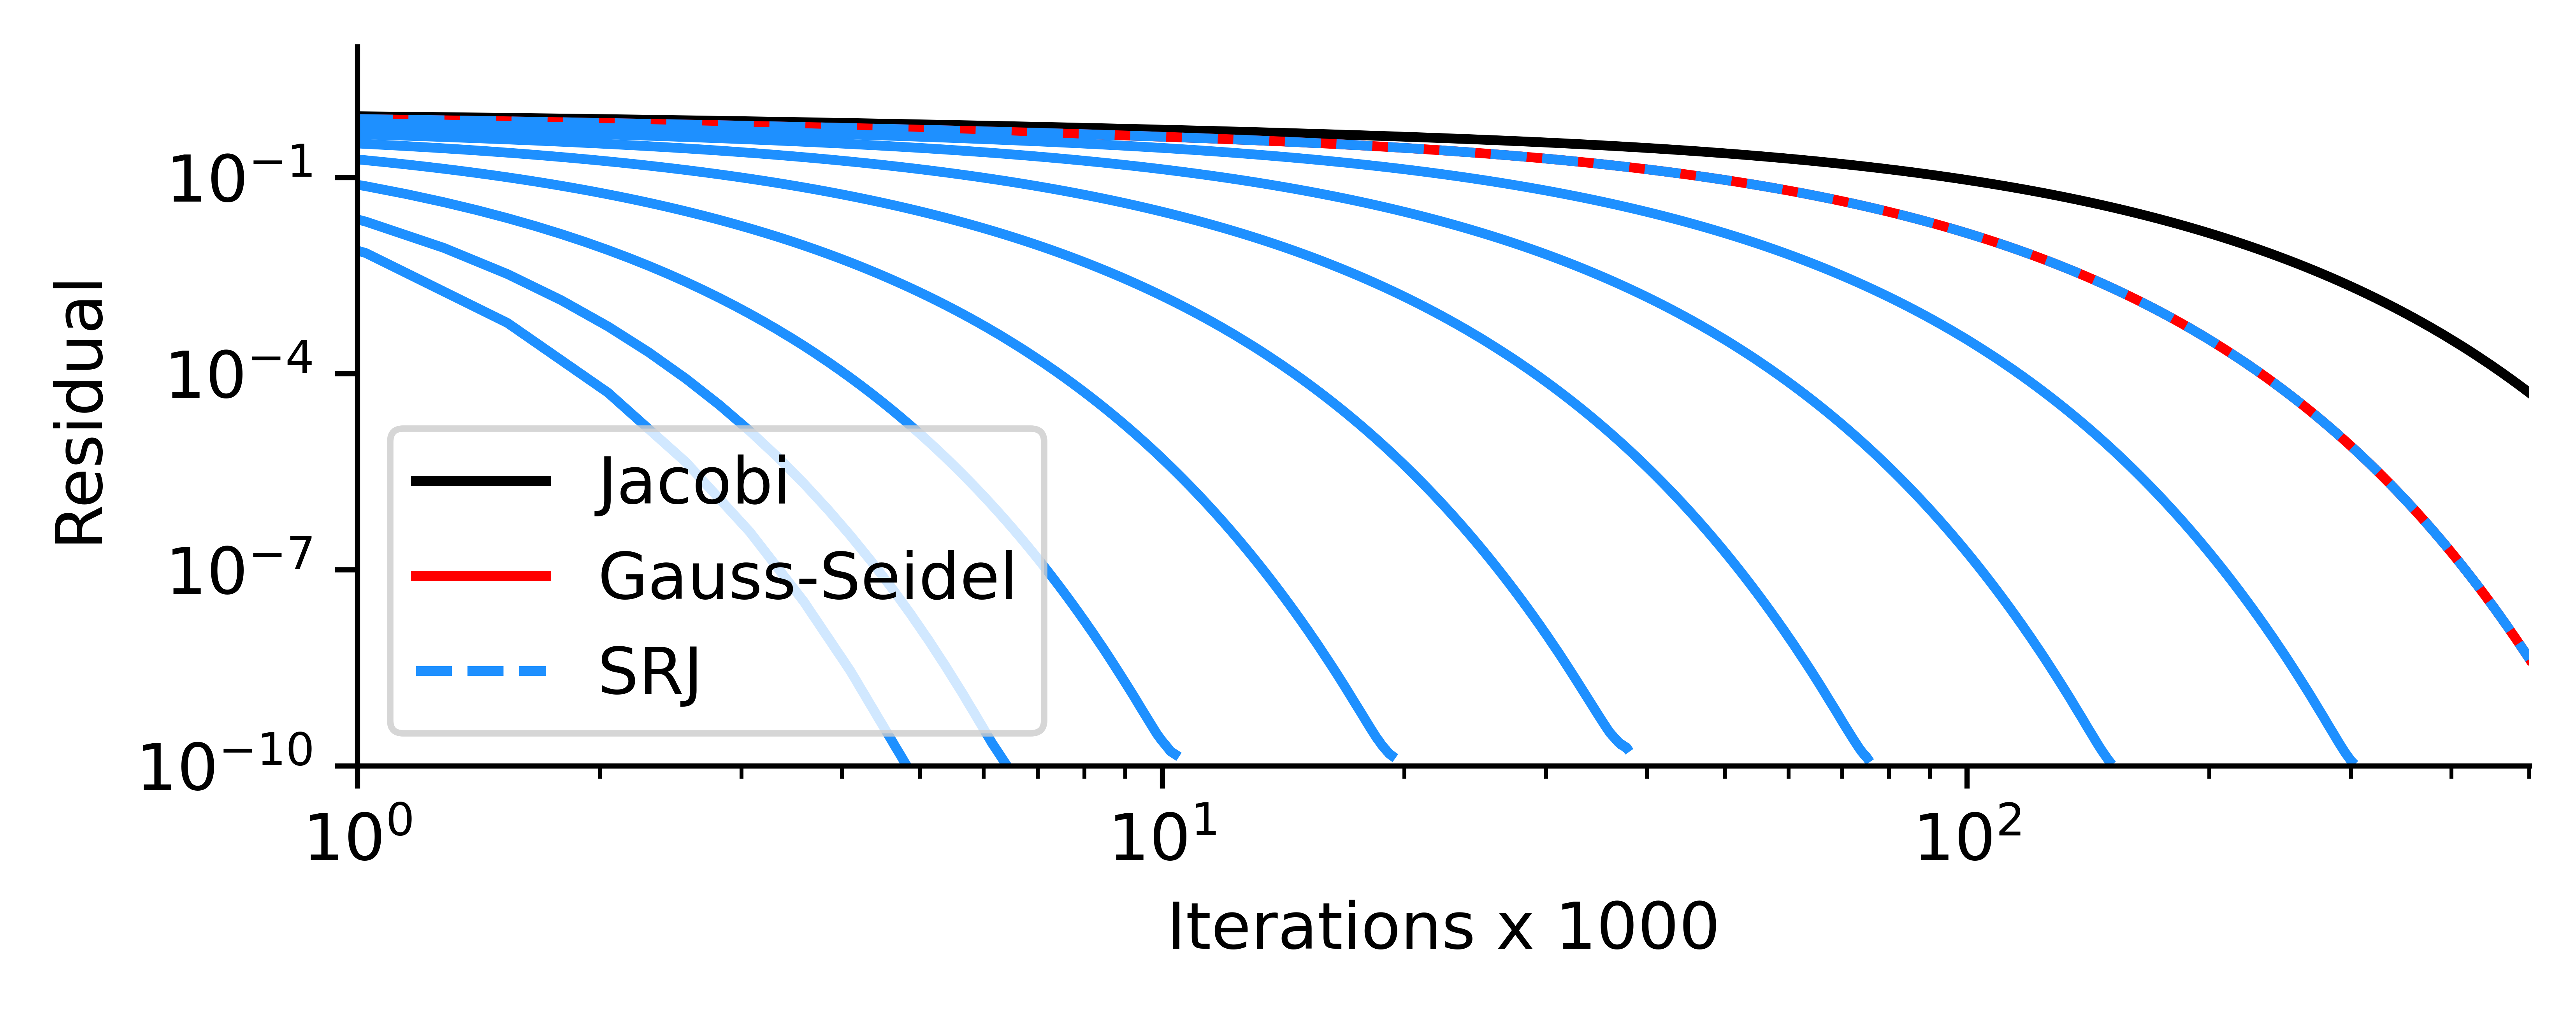
\includegraphics[width=\textwidth]{comparaisons_2D_logscale}
    \vfill
  \end{frame}
}

{
  \setbeamercolor{background canvas}{bg=white}
  \begin{frame}[fragile]{}{}
    \vfill
    \centering
    \huge
    \textbf{\color{black} Conclusion}
    \vfill
  \end{frame}
}

\begin{frame}
  Despite what is classicaly taught, Jacobi-based methods can be massively accelerated by combining \textbf{over-relaxations} and \textbf{under-relaxations}.
  
  \pause
  
  \bigskip
  
  To this day, \textbf{Scheduled-Relaxation Jacobi} can achieve performances comparable to other efficient iterative solvers, making it a competitive alternative.
  
  \pause
  
  \bigskip
  
  One major advantage of \textbf{SRJ} is that it retains the easy implementation and straightforward parallelisation of the original Jacobi method.
  
  \vspace{-1cm}
\end{frame}

\begin{frame}
  \textbf{SRJ} can be used as direct replacement of Jacobi preconditionner for Krylov methods such as \textbf{GMRES} or \textbf{PCG}.
  It can also be used \emph{in lieu} of Jacobi or Gauss-Seidel smoothing for multigrid methods (e.g. \textbf{AMG}).

  \vspace{-1cm}
\end{frame}


{
  \setbeamercolor{background canvas}{bg=white}
  \begin{frame}[fragile]{}{}
    \vfill
    \flushright
    \Large
    \textbf{\color{black} Thank for your attention}

    \large
    \textbf{\color{gray} Any question ?}
    \vfill
  \end{frame}
}

\end{document}
